%  A simple AAU report template.
%  2015-05-08 v. 1.2.0
%  Copyright 2010-2015 by Jesper Kjær Nielsen <jkn@es.aau.dk>
%
%  This is free software: you can redistribute it and/or modify
%  it under the terms of the GNU General Public License as published by
%  the Free Software Foundation, either version 3 of the License, or
%  (at your option) any later version.
%
%  This is distributed in the hope that it will be useful,
%  but WITHOUT ANY WARRANTY; without even the implied warranty of
%  MERCHANTABILITY or FITNESS FOR A PARTICULAR PURPOSE.  See the
%  GNU General Public License for more details.
%
%  You can find the GNU General Public License at <http://www.gnu.org/licenses/>.
%
%  A simple AAU report template.
%  2015-05-08 v. 1.2.0
%  Copyright 2010-2015 by Jesper Kjær Nielsen <jkn@es.aau.dk>
%
%  This is free software: you can redistribute it and/or modify
%  it under the terms of the GNU General Public License as published by
%  the Free Software Foundation, either version 3 of the License, or
%  (at your option) any later version.
%
%  This is distributed in the hope that it will be useful,
%  but WITHOUT ANY WARRANTY; without even the implied warranty of
%  MERCHANTABILITY or FITNESS FOR A PARTICULAR PURPOSE.  See the
%  GNU General Public License for more details.
%
%  You can find the GNU General Public License at <http://www.gnu.org/licenses/>.
%
\documentclass[11pt,twoside,a4paper,openright]{report}
%%%%%%%%%%%%%%%%%%%%%%%%%%%%%%%%%%%%%%%%%%%%%%%%
% Language, Encoding and Fonts
% http://en.wikibooks.org/wiki/LaTeX/Internationalization
%%%%%%%%%%%%%%%%%%%%%%%%%%%%%%%%%%%%%%%%%%%%%%%%
% Select encoding of your inputs. Depends on
% your operating system and its default input
% encoding. Typically, you should use
%   Linux  : utf8 (most modern Linux distributions)
%            latin1 
%   Windows: ansinew
%            latin1 (works in most cases)
%   Mac    : applemac
% Notice that you can manually change the input
% encoding of your files by selecting "save as"
% an select the desired input encoding. 
\usepackage[utf8]{inputenc}
% Make latex understand and use the typographic
% rules of the language used in the document.
\usepackage[danish,english]{babel}
% Use the palatino font
\usepackage[sc]{mathpazo}
\linespread{1.05}         % Palatino needs more leading (space between lines)
% Choose the font encoding
\usepackage[T1]{fontenc}
%%%%%%%%%%%%%%%%%%%%%%%%%%%%%%%%%%%%%%%%%%%%%%%%
% Graphics and Tables
% http://en.wikibooks.org/wiki/LaTeX/Importing_Graphics
% http://en.wikibooks.org/wiki/LaTeX/Tables
% http://en.wikibooks.org/wiki/LaTeX/Colors
%%%%%%%%%%%%%%%%%%%%%%%%%%%%%%%%%%%%%%%%%%%%%%%%
% load a colour package
\usepackage{xcolor}
\definecolor{aaublue}{RGB}{33,26,82}% dark blue
% The standard graphics inclusion package
\usepackage{graphicx}
% Set up how figure and table captions are displayed
\usepackage{caption}
\captionsetup{%
  font=footnotesize,% set font size to footnotesize
  labelfont=bf % bold label (e.g., Figure 3.2) font
}
% Make the standard latex tables look so much better
\usepackage{array,booktabs}
% Enable the use of frames around, e.g., theorems
% The framed package is used in the example environment
\usepackage{framed}

%%%%%%%%%%%%%%%%%%%%%%%%%%%%%%%%%%%%%%%%%%%%%%%%
% Mathematics
% http://en.wikibooks.org/wiki/LaTeX/Mathematics
%%%%%%%%%%%%%%%%%%%%%%%%%%%%%%%%%%%%%%%%%%%%%%%%
% Defines new environments such as equation,
% align and split 
\usepackage{amsmath}
% Adds new math symbols
\usepackage{amssymb}
% Use theorems in your document
% The ntheorem package is also used for the example environment
% When using thmmarks, amsmath must be an option as well. Otherwise \eqref doesn't work anymore.
\usepackage[framed,amsmath,thmmarks]{ntheorem}

%%%%%%%%%%%%%%%%%%%%%%%%%%%%%%%%%%%%%%%%%%%%%%%%
% Page Layout
% http://en.wikibooks.org/wiki/LaTeX/Page_Layout
%%%%%%%%%%%%%%%%%%%%%%%%%%%%%%%%%%%%%%%%%%%%%%%%
% Change margins, papersize, etc of the document
\usepackage[
  inner=28mm,% left margin on an odd page
  outer=41mm,% right margin on an odd page
  %top=,
  %bottom=,
  ]{geometry}
% Modify how \chapter, \section, etc. look
% The titlesec package is very configureable
\usepackage{titlesec}
\titleformat{\chapter}[display]{\normalfont\huge\bfseries}{\chaptertitlename\ \thechapter}{20pt}{\Huge}
\titleformat*{\section}{\normalfont\Large\bfseries}
\titleformat*{\subsection}{\normalfont\large\bfseries}
\titleformat*{\subsubsection}{\normalfont\normalsize\bfseries}
%\titleformat*{\paragraph}{\normalfont\normalsize\bfseries}
%\titleformat*{\subparagraph}{\normalfont\normalsize\bfseries}

% Clear empty pages between chapters
\let\origdoublepage\cleardoublepage
\newcommand{\clearemptydoublepage}{%
  \clearpage
  {\pagestyle{empty}\origdoublepage}%
}
\let\cleardoublepage\clearemptydoublepage

% Change the headers and footers
\usepackage{fancyhdr}
\pagestyle{fancy}
\fancyhf{} %delete everything
\renewcommand{\headrulewidth}{0pt} %remove the horizontal line in the header
\fancyhead[RE]{\small\nouppercase\leftmark} %even page - chapter title
\fancyhead[LO]{\small\nouppercase\rightmark} %uneven page - section title
\fancyhead[LE,RO]{\thepage} %page number on all pages, header
% \fancyfoot[LE,RO]{Page \thepage\space of \pageref{LastPage}} %page number on all pages, footer
% Do not stretch the content of a page. Instead,
% insert white space at the bottom of the page
\raggedbottom
% Enable arithmetics with length. Useful when
% typesetting the layout.
\usepackage{calc}

%%%%%%%%%%%%%%%%%%%%%%%%%%%%%%%%%%%%%%%%%%%%%%%%
% Bibliography
% http://en.wikibooks.org/wiki/LaTeX/Bibliography_Management
%%%%%%%%%%%%%%%%%%%%%%%%%%%%%%%%%%%%%%%%%%%%%%%%
%\usepackage[backend=biber,
%  bibencoding=utf8,
%  style=numeric,
%  sorting = none,
%  %citestyle=apa,
%  language=danish,
%  ]{biblatex}
%\usepackage{url}


\usepackage[square]{natbib}

\bibliographystyle{unsrtnat} % viser referencers url

\usepackage[hyphens]{url} % url formatering
\usepackage{hyperref}

%\usepackage{babel/polyglossia}
\usepackage{csquotes}

%%%%%%%%%%%%%%%%%%%%%%%%%%%%%%%%%%%%%%%%%%%%%%%%
% Misc
%%%%%%%%%%%%%%%%%%%%%%%%%%%%%%%%%%%%%%%%%%%%%%%%
% Add bibliography and index to the table of
% contents
\usepackage[nottoc]{tocbibind}
% Add the command \pageref{LastPage} which refers to the
% page number of the last page
\usepackage{lastpage}
% Add todo notes in the margin of the document
\usepackage[
%  disable, %turn off todonotes
  colorinlistoftodos, %enable a coloured square in the list of todos
  textwidth=\marginparwidth, %set the width of the todonotes
  textsize=scriptsize, %size of the text in the todonotes
  ]{todonotes}

%%%%%%%%%%%%%%%%%%%%%%%%%%%%%%%%%%%%%%%%%%%%%%%%
% Hyperlinks
% http://en.wikibooks.org/wiki/LaTeX/Hyperlinks
%%%%%%%%%%%%%%%%%%%%%%%%%%%%%%%%%%%%%%%%%%%%%%%%
% Enable hyperlinks and insert info into the pdf
% file. Hypperref should be loaded as one of the 
% last packages
\usepackage{hyperref}
\hypersetup{%
	plainpages=false,%
	pdfauthor={Author(s)},%
	pdftitle={Title},%
	pdfsubject={Subject},%
	bookmarksnumbered=true,%
	colorlinks=false,%
	citecolor=black,%
	filecolor=black,%
	linkcolor=black,% you should probably change this to black before printing
	urlcolor=black,%
	pdfstartview=FitH%
}


% skriv \par for halvt linieskift 
\setlength{\parindent}{0em}    %bestemmer indrykning på linie
\setlength{\parskip}{0.5em}    %bestemmer størrelse af linieskift

\usepackage{float}
\usepackage{booktabs}
\usepackage{enumitem}

\usepackage{amssymb}

\usepackage{longtable}

\usepackage{makecell}

\newlength\mytemplength

\newcommand\parboxc[3]{%
    \settowidth{\mytemplength}{#3}%
    \parbox[#1][#2]{\mytemplength}{\centering #3}%
}


\usepackage{listings}

%Coding:
\usepackage[newfloat]{minted}
\usepackage{caption}
\newenvironment{code}{\captionsetup{type=listing}}{}
\SetupFloatingEnvironment{listing}{name=Code example}

\usepackage{csquotes}

% Viser mere info om fejl
%\setcounter{errorcontextlines}{999}% package inclusion and set up of the document
% see, e.g., http://en.wikibooks.org/wiki/LaTeX/Formatting#Hyphenation
% for more information on word hyphenation
\hyphenation{ex-am-ple hy-phen-a-tion short}
\hyphenation{long la-tex}
% 
%  A simple AAU report template.
%  2015-05-08 v. 1.2.0
%  Copyright 2010-2015 by Jesper Kjær Nielsen <jkn@es.aau.dk>
%
%  This is free software: you can redistribute it and/or modify
%  it under the terms of the GNU General Public License as published by
%  the Free Software Foundation, either version 3 of the License, or
%  (at your option) any later version.
%
%  This is distributed in the hope that it will be useful,
%  but WITHOUT ANY WARRANTY; without even the implied warranty of
%  MERCHANTABILITY or FITNESS FOR A PARTICULAR PURPOSE.  See the
%  GNU General Public License for more details.
%
%  You can find the GNU General Public License at <http://www.gnu.org/licenses/>.
%
%
%
% see, e.g., http://en.wikibooks.org/wiki/LaTeX/Customizing_LaTeX#New_commands
% for more information on how to create macros

\DeclareCaptionType{use_case}[Use Case]
\DeclareCaptionType{actor}[Actor]

%%%%%%%%%%%%%%%%%%%%%%%%%%%%%%%%%%%%%%%%%%%%%%%%
% Macros for the titlepage
%%%%%%%%%%%%%%%%%%%%%%%%%%%%%%%%%%%%%%%%%%%%%%%%
%Creates the aau titlepage
\newcommand{\aautitlepage}[3]{%
  {
    %set up various length
    \ifx\titlepageleftcolumnwidth\undefined
      \newlength{\titlepageleftcolumnwidth}
      \newlength{\titlepagerightcolumnwidth}
    \fi
    \setlength{\titlepageleftcolumnwidth}{0.5\textwidth-\tabcolsep}
    \setlength{\titlepagerightcolumnwidth}{\textwidth-2\tabcolsep-\titlepageleftcolumnwidth}
    %create title page
    \thispagestyle{empty}
    \noindent%
    \begin{tabular}{@{}ll@{}}
      \parbox{\titlepageleftcolumnwidth}{
        \iflanguage{danish}{%
          
\includegraphics[width=\titlepageleftcolumnwidth]{figures/aau_logo_da}
        }{%
          
\includegraphics[width=\titlepageleftcolumnwidth]{figures/aau_logo_en}
        }
      } &
      \parbox{\titlepagerightcolumnwidth}{\raggedleft\sf\small
        #2
      }\bigskip\\
       #1 &
      \parbox[t]{\titlepagerightcolumnwidth}{%
      \textbf{Abstract:}\bigskip\par
        \fbox{\parbox{\titlepagerightcolumnwidth-2\fboxsep-2\fboxrule}{%
          #3
        }}
      }\\
    \end{tabular}
    \vfill
    \iflanguage{danish}{%
      \noindent{\footnotesize\emph{Rapportens indhold er frit tilgængeligt, men offentliggørelse (med kildeangivelse) må kun ske efter aftale med forfatterne.}}
    }{%
      \noindent{\footnotesize\emph{The content of this report is freely available, but publication (with reference) may only be pursued due to agreement with the author.}}
    }
    \clearpage
  }
}

%Create english project info
\newcommand{\englishprojectinfo}[8]{%
  \parbox[t]{\titlepageleftcolumnwidth}{
    \textbf{Title:}\\ #1\bigskip\par
    \textbf{Theme:}\\ #2\bigskip\par
    \textbf{Project Period:}\\ #3\bigskip\par
    \textbf{Project Group:}\\ #4\bigskip\par
    \textbf{Participant(s):}\\ #5\bigskip\par
    \textbf{Supervisor(s):}\\ #6\bigskip\par
    %\textbf{Copies:} #7\bigskip\par
    \textbf{Page Numbers:} \pageref{LastPage}\bigskip\par
    \textbf{Date of Completion:}\\ #8
  }
}

%Create danish project info
\newcommand{\danishprojectinfo}[8]{%
  \parbox[t]{\titlepageleftcolumnwidth}{
    \textbf{Titel:}\\ #1\bigskip\par
    \textbf{Tema:}\\ #2\bigskip\par
    \textbf{Projektperiode:}\\ #3\bigskip\par
    \textbf{Projektgruppe:}\\ #4\bigskip\par
    \textbf{Deltager(e):}\\ #5\bigskip\par
    \textbf{Vejleder(e):}\\ #6\bigskip\par
    \textbf{Oplagstal:} #7\bigskip\par
    \textbf{Sidetal:} \pageref{LastPage}\bigskip\par
    \textbf{Afleveringsdato:}\\ #8
  }
}

%%%%%%%%%%%%%%%%%%%%%%%%%%%%%%%%%%%%%%%%%%%%%%%%
% An example environment
%%%%%%%%%%%%%%%%%%%%%%%%%%%%%%%%%%%%%%%%%%%%%%%%
\theoremheaderfont{\normalfont\bfseries}
\theorembodyfont{\normalfont}
\theoremstyle{break}
\def\theoremframecommand{{\color{gray!50}\vrule width 5pt \hspace{5pt}}}
\newshadedtheorem{exa}{Example}[chapter]
\newenvironment{example}[1]{%
		\begin{exa}[#1]
}{%
		\end{exa}
}
% my new macros

\begin{document}
%frontmatter
\pagestyle{empty} %disable headers and footers
\pagenumbering{roman} %use roman page numbering in the frontmatter
%  A simple AAU report template.
%  2015-05-08 v. 1.2.0
%  Copyright 2010-2015 by Jesper Kjær Nielsen <jkn@es.aau.dk>
%
%  This is free software: you can redistribute it and/or modify
%  it under the terms of the GNU General Public License as published by
%  the Free Software Foundation, either version 3 of the License, or
%  (at your option) any later version.
%
%  This is distributed in the hope that it will be useful,
%  but WITHOUT ANY WARRANTY; without even the implied warranty of
%  MERCHANTABILITY or FITNESS FOR A PARTICULAR PURPOSE.  See the
%  GNU General Public License for more details.
%
%  You can find the GNU General Public License at <http://www.gnu.org/licenses/>.
%
\pdfbookmark[0]{Front page}{label:frontpage}%
\begin{titlepage}
  \addtolength{\hoffset}{0.5\evensidemargin-0.5\oddsidemargin} %set equal margins on the frontpage - remove this line if you want default margins
  \noindent%
  \begin{tabular}{@{}p{\textwidth}@{}}
    \toprule[2pt]
    \midrule
    \vspace{0.2cm}
    \begin{center}
    \Huge{\textbf{
      Asset Management System% insert your title here
    }}
    \end{center}
    \begin{center}
      \Large{
        The development of the Asset Management System% insert your subtitle here
      }
    \end{center}
    \vspace{0.2cm}\\
    \midrule
    \toprule[2pt]
  \end{tabular}
  \vspace{4 cm}
  \begin{center}
    {\large
      P3 Project Paper%Insert document type (e.g., Project Report)
    }\\
    \vspace{0.2cm}
    {\Large
      DS303E19%Insert your group name or real names here
    }
  \end{center}
  \vfill
  \begin{center}
  Aalborg University\\
  Computer Science
  \end{center}
\end{titlepage}
\clearpage

\newgeometry{top=20mm, bottom=20mm}
    \thispagestyle{empty}
{\small
\strut\vfill % push the content to the bottom of the page
\noindent Copyright \copyright{} Aalborg University 2019\par
\vspace{0.2cm}
\noindent Here you can write something about which tools and software you have used for typesetting the document, running simulations and creating figures. If you do not know what to write, either leave this page blank or have a look at the colophon in some of your books.
}
\clearpage


    \pdfbookmark[0]{English title page}{label:titlepage_en}
\aautitlepage{%
  \englishprojectinfo{
    Asset Management System %title
  }{%
    Company Communication %theme
  }{%
    Fall Semester 2019 %project period
  }{%
    DS303E19 % project group
  }{%
    %list of group members
    Alexander Nykjær\\
    Ane Søgaard Jørgensen\\
    Daniel Fly\\ 
    Jakob Sønderby Kristensen\\
    Michelle Volf Terpling\\
    Niels Vistisen\\
    Thomas Lorentzen
  }{%
    %list of supervisors
    Lu Chen
  }{
    
  }{%
    \today % date of completion
  }%
}{%department and address
  \textbf{Computer Science}\\
  Aalborg University\\
  \href{http://www.aau.dk}{http://www.aau.dk}
}{% the abstract
    
\begin{verbatim}
        o                o         
                               o     
          o          O            
                ______    o      
              _/  (   \_        
    _       _/  (       \_   O      
    | \_   _/  (   (    0  \        
    |== \_/  (   (          |      
    |=== _ (   (   (        |       
    |==_/ \_ (   (          |     
    |_/     \_ (   (    \__/    
             \_ (      _/         
               |  |___/          
              /__/               
\end{verbatim}
    
}

\restoregeometry
\cleardoublepage
\pdfbookmark[0]{Contents}{label:contents}
\pagestyle{fancy} %enable headers and footers again
\tableofcontents
\listoftodos \todo[inline] {Fjern den her!} 
\chapter*{Preface\markboth{Preface}{Preface}}\label{ch:preface}
\addcontentsline{toc}{chapter}{Preface}
Here is the preface. You should put your signatures at the end of the preface.

\subsection*{Reading Guide}

\vspace{\baselineskip}\hfill Aalborg University, \today
\vfill\noindent
\vspace{0.5\baselineskip}
\begin{minipage}[b]{0.45\textwidth}
 \centering
 \rule{\textwidth}{0.5pt}\\
  Alexander Nykjær\\
 {\footnotesize <anykjal18@student.aau.dk>}
\end{minipage}
\hfill
\begin{minipage}[b]{0.45\textwidth}
 \centering
 \rule{\textwidth}{0.5pt}\\
  Ane Søgaaard Jørgensen\\
 {\footnotesize <asja18@student.aau.dk>}
\end{minipage}

\vspace{1\baselineskip}
\begin{minipage}[b]{0.45\textwidth}
 \centering
 \rule{\textwidth}{0.5pt}\\
  Daniel Fly\\
 {\footnotesize <dfly18@student.aau.dk>}
\end{minipage}
\hfill
\begin{minipage}[b]{0.45\textwidth}
 \centering
 \rule{\textwidth}{0.5pt}\\
  Jakob Sønderby Kristensen\\
 {\footnotesize <jkr18@student.aau.dk>}
\end{minipage}

\vspace{1\baselineskip}
\begin{minipage}[b]{0.45\textwidth}
 \centering
 \rule{\textwidth}{0.5pt}\\
  Michelle Volf Terpling\\
 {\footnotesize <mterpl18@student.aau.dk>}
\end{minipage}
\hfill
\begin{minipage}[b]{0.45\textwidth}
 \centering
 \rule{\textwidth}{0.5pt}\\
  Niels Vistisen \\
 {\footnotesize <nvisti18@student.aau.dk>}
\end{minipage}

%\vspace{3.5\baselineskip}
% 
\vspace{0.8\baselineskip}
\begin{center}
\begin{minipage}[b]{0.45\textwidth}
 \centering
 \rule{\textwidth}{0.5pt}\\
  Thomas Lorentzen\\
 {\footnotesize <tglo18@student.aau.dk>}
\end{minipage}
\end{center}
\cleardoublepage
%mainmatter
\pagenumbering{arabic} %use arabic page numbering in the mainmatter

%%%%%%%%%%%%%%%%%%%%%%%%%%%%%%%%%%%%%%%%%%%%%%%%%%%%%%%%%%%%%%%
%%%%%%%%%%%%%%%%%%%%%%%%%%%%%%%%%%%%%%%%%%%%%%%%%%%%%%%%%%%%%%%
% Introduction to the report
\chapter{Introduction}\label{ch:introduction}
As companies expand and acquire a growing number of assets, the desire to keep track of these assets and their condition can also grow \citep{ImportanceOfAM}. Creating an overview of the assets, and keeping this overview up to date, is a major task and one that companies sometimes do not address until the number of assets in their possession has become overwhelming \citep{DoNotIgnoreSAM}. These issues are clear when looking at the growing market of asset management software. The submarket of digital asset managements is estimated to grow from 1.2 billion in 2018, to 6,901 billion by 2024 \citep{MarketGrowth}.
\par
While there are many existing solutions, these are often very extensive and try to accommodate a lot of different use cases by adding more data points to the design \citep{SnipeIT}. This can however lead to the system becoming overwhelming itself. A way of making a solution more suitable for a wide range of companies while still keeping it simple, could be to make it more adaptable \citep{CustomSoftware}. With this approach, the individual company will not be overwhelmed with unneeded User Interface (UI) elements, that are only relevant for a few specific companies.
\par
Focusing on a specific department at a specific company, has limited the magnitude of the project. The collaborator of this project has been the IT department at Aalborg Zoo. Therefore, the specific needs of Aalborg Zoo has been a high priority, as they are considered the customer of the finished product.
\par
Aalborg Zoo is located in the center of Aalborg, and welcomes around 341.000 visitors each year \citep{AalborgZoo}. The zoo has 44 employees with different backgrounds and responsibilities \citep{AalborgZoo}. Because of this, the zoo is divided into multiple departments \citep{PersonaleAZ}. The IT department has multiple responsibilities, including supplying the other departments with computers, walkie talkies, routers, and more (see \autoref{sc:aalborgZoo}). In line with the growth of the zoo and technological advancements, the IT department has come in charge of a lot of different assets. These assets can be loaned out to any employee or department at any point, which can make it hard to keep track of their locations and conditions.
\par
To accommodate this growing task and to ensure an overview of the assets, the IT department has requested an asset management system.

\subsubsection*{Problem statement}
Based on the mentioned issues with existing solutions to the problem, the following problem statement has been formulated and used as the main focus of the project.

\begin{quote}
    \textit{How can a system be designed to be more adaptable than existing asset management systems?}
\end{quote}

% How can a system help Aalborg Zoo manage their assets better than existing tools can?

% How can a system be created to help the IT department at Aalborg Zoo manage their assets?

% How to develop a software system to help the IT department at Aalborg Zoo to manage their systems?

% How can a system, that helps Aalborg Zoo manage their assets, be designed and implemented?

% How can a software solution help manage Aalborg Zoo's assets?




% Background
\chapter{Background}\label{ch:background}
% alternative titler: Purpose
In this chapter the background and purpose of this project will be described. The client, Aalborg Zoo, will be introduced and their problem described. Based on this a list of requirements and a system definition will be defined. 
\section{Aalborg Zoo}\label{ch:problemdefinition}
Focusing on a specific department at a specific company, has limited the magnitude of the project. The collaborator of this project has been the IT department at Aalborg Zoo, who asked for an Asset Management System that is more dynamic than the existing solutions. Therefore, the needs of Aalborg Zoo has been a high priority, as they have been seen as the customer of the finished product.
\par
The collaboration has been based on a series of semi-structured interviews, which have been conducted with the head of the IT department, Morten Rom, and technician Kasper Andersen who make up the IT department at Aalborg Zoo, and have been representatives of the IT department and partly the zoo as a whole. They have described a problem with keeping track of and maintaining assets within the zoo due to the physical size of the zoo and the number of different assets, departments, and employees. Their system for managing their assets has been to type in information that was thought relevant, in an excel document, at the point of acquisition. This system is flawed, as the pieces of information added by different employees change from time to time, and information about the assets is not being kept up to date. Therefore, a proper Asset Management System could be a good addition to the company.
\par
During the interviews, the representatives were asked, if they had looked for alternatives, as systems solving the problem already exists. To this they answered that the existing solutions provide too many required and predefined fields. Here a field could be a textbox, checkbox, date field, etc., meant to contain information about the asset. Instead they wanted a dynamic system with only the information they needed for every specific asset, resulting in a cleaner, more manageable interface for managing assets.
\par
They have expressed interest in logging changes, made to assets, and the ability to export a list of assets as well as the log. 


\todo[inline]{Overgang til problemformuleringen}



% Knowing the location of each individual assets comes down to the different employees in the zoo. As a result, no one has a clear picture of the assets within the zoo. Therefore Aalborg Zoo has been looking at different asset management systems. Currently they do not have the resources to develop such a system for themselves, and has examined other options. However, none of these satisfy their requirements. They want a program that is cheap and easy to use, without presenting the user with a large number of fields to fill out for each new entry into the system. 

%\begin{itemize}
%    \item Make it possible for an administrator to record when employees borrow assets, or associate an asset with a location. This should be done by adding special tags, like a user or location tag.
    
%    \item Add uncategorized tags with additional relevant information to assets. This could be the status of the asset, if for example it is under maintenance. 
    
%    \item A log of the changes made to assets, along with information about who made the change and when it was made. It should also be logged when an asset is added or removed. 
    
%    \item Templates for assets, with only the necessary fields that all assets of that template need to have. For example a switch needs fields with ID, IP-address, and password. All other relevant information can be added through tags.
%\end{itemize}

%The reason for the small number of required fields, is due to the clients wishes. They expressed a dislike for other asset management systems that required too many fields to be filled for each asset. They also wanted as few clicks of the mouse as possible.
\section{Problem Definition}
Based on the interviews with Aalborg Zoo, the following problem definition has been formulated:

\begin{quote}
    \textit{The IT department at Aalborg Zoo has many assets and no sufficient system to manage the assets.}
\end{quote}

\begin{quote}
    \textit{How can a system help Aalborg Zoo manage their assets better than existing tools can?}
    
    How can a system be created to help the IT department at Aalborg Zoo manage their assets?
    
    How to develop a software system to help the IT department at Aalborg Zoo to manage their systems?
    
    How can a system, that helps Aalborg Zoo manage their assets, be designed and implemented?
    
    How can a software solution help manage Aalborg Zoo's assets?
\end{quote}

They have not been able to find a viable solution among existing products. It is the goal of this project to develop such a solution. 
\par
To ensure that the representatives of Aalborg Zoo and the project group all agree on the extent of the project, a system definition has been developed based on the interviews from which a list of requirements have been made.
\section{Requirements}\label{sc:requirements}
Based on the interviews with the zoo and on the analysis above, a list of requirements have been formulated. According to the MoSCoW \cite[chap 7.1]{DEB} method, these requirements have been divided into categories based on their priority. The final requirement specification can be seen in the following table (table \ref{tab:moscow}). This prioritisation has been approved by the client and will dictate the development of the system. 

\begin{longtable}{p{3.2cm} p{10cm}}
    \renewcommand{\arraystretch}{2.0}
        \\
        \hline
        \textbf{Must have} & 
        \vspace*{-7mm}
        \begin{enumerate} \itemsep0em 
            \item Assets can be added, removed, and edited.
            \item It will be possible to search through all assets with either identifier or name.
            \item Information on users will be imported from the Active Directory, through a CSV file.
        \end{enumerate}
        \\
        \hline
        
        \textbf{Should have} & 
        \vspace*{-7mm}
        \begin{enumerate} \setcounter{enumi}{3} \itemsep0em 
            \item Assets and log entries can be exported to a file based on a search.
            \item Admins and viewers can add comments to assets. Admins can remove and edit all comments, while viewers can only edit their own comments.
            \item Comments for each asset will be accessible from within the specific asset.
            \item All changes to assets, tags, and comments will be logged.
            \item Fields will be set to a certain type and can be marked as required. It will be possible for a field to have a default value.
            \item The design will be very minimalist.
            \item Tags will be presented in different colors. Subtags will inherit the color of their parent tag. Colors will be assigned randomly if not chosen by the user.
        \end{enumerate}
        \\
        \hline
        
        \textbf{Nice to have} &     
        \vspace*{-7mm}
        \begin{enumerate} \setcounter{enumi}{10} \itemsep0em 
            \item Departments can be added, removed, and edited. Each user can set their default department.
            
            \item Tags are department specific.
            
            \item It will be possible to select multiple assets or select all and then deselect certain assets. The selected assets can then be exported to a file.
            
            \item When searching for assets, a list of tags on the found assets will be shown. From this list it will be possible to hide assets by deselecting tags.
            
            \item Assets can expire, and the system should inform the user of this.
            
            \item Notifications will be based on function tags.
            
            \item Viewers can request an asset. The admins can view, approve, or deny all requests for assets.
            
        \end{enumerate}
        \\
        \hline
        \textbf{Won't have this time} & 
        \vspace*{-7mm}
        \begin{enumerate} \setcounter{enumi}{17} \itemsep0em 
            \item AND, OR, and parentheses can be used to enable complex searching.
            \item System functions can be linked to barcodes.
        \end{enumerate}
        \\
        \hline
    \caption{MoSCoW}
    \label{tab:moscow}
   
\end{longtable}
\section{System Definition}\label{sc:SystemDefinition}
The primary functionality of the system is to give the user the ability to add, edit, remove, and search through all assets. The search will be based on the assets' unique IDs, names, or identifiers specified by the user, such as tags and fields, and is limited to the selected department. When adding a new asset to the system, the user will be able to add predefined tags to the asset. These tags can contain fields that should be filled out for the specific assets.
\par
The system will have the functionality to tag assets with attributes such as their location and the person borrowing the asset. The user will be able to add new tags to the system and assign these to parent tags. The parent tags will act as tag categories, which the user can define. 
\par
Another functionality of the system is logging changes. The system will be able to provide a history of events for each asset. These include adding an asset, editing an asset, and attaching and detaching tags to an asset. The user will also be able to add comments to assets, describing events such as updating the operating system of a computer or installing new software to an asset. Every event and comment will have the username of the person who made the change attached.
\par
The system is developed to be primarily used by the IT department, and has a group of users who can manage the system, logging in automatically using their Active Directory (AD) identity. Other departments will also have access to the system. All employees will be able to view and comment on the assets, but only the assigned administrators will have the ability to manage them. 
\par
The interface will be simple and easy to use, changing the search results based on the selected department. The user will be able to generate a list of assets and export it to a file.
\par
The system will be programmed using the C\# language and will be developed for a Windows PC. The system will be communicating with a database and have a graphical user interface.
\par
The primary objects in the problem domain are:
\begin{itemize}
    \item \textbf{Asset}: Corporate assets in Aalborg Zoo, such as computers, switches, phones, etc.
    
    \item \textbf{Employee}: Every employee can access the system and see every asset. Some employees can be granted further access to functionality, at which point they become an admin.
    
    \item \textbf{Admin}: Users with authority to manage and lend assets to other employees.
    
    \item \textbf{Department}: Different departments within the zoo, which oversee multiple assets.
\end{itemize}
While tags are an essential part of the system, they are not objects in the problem domain and will not be discussed again till \autoref{sc:model_component}.
\par
A more concise version of the system definition can be found in the appendix as a FACTOR criterion (see \autoref{app:factor}).
\subsection*{FACTOR} \label{sec:factor}
\par
\begin{table}[H]
    \centering
    {
    \renewcommand{\arraystretch}{2.0}
    \begin{tabular}{ m{4cm} m{10cm} }
        \hline
        
        \textbf{Functions} & A system to keep track of the zoo's assets with the ability to add, edit and delete assets. Furthermore, the system should offer the ability to add custom tags to ease the process of adding new assets to the system and updating attributes such as their condition, location, and the person currently in possession of the asset. All interactions will be logged, to ensure a backup of changed values, if a mistake is made. The system should also offer the ability to search through and exporting a list of assets and the log.\\
        
        \textbf{Application Domain} & The system will be administrated and used by the IT department at Aalborg Zoo, but other departments can also use the system to see the assets.\\
        
        \textbf{Conditions} & The system will be used by the IT department, who has experience with computers and servers. The client has requested a simple user interface with only as many elements as needed. The system will run on a windows PC and might be brought around the premises of the zoo.\\
        
        \textbf{Technology} & The system will be run on different PC's (including laptops), which can vary in age. The PC's will be equipped with current tools. The system will be programmed in C\# and communicate with a MySQL server.\\
        
        \textbf{Objects} & Asset, admin, and employee.\\
        
        \textbf{Responsibilities} & The system should be able to keep track of assets and give the IT-department an overview of their assets. The system should also be able to export a list of assets.\\
        
        \hline
    \end{tabular}
    \caption{FACTOR Criterion for the system}
    \label{tab:factor}
    }
\end{table}
\section{Method}
% Processor!
The project has been produced as a group project with a group of seven members. Throughout the project period, multiple courses has been attended by the members on a weekly basis, and these courses has been an academic basis for the entire project. The courses have taken time from the project work, but has contributed irreplaceable knowledge to its group members. The time not spent on courses has been used to develop this report and the product system.
\par
To ensure the quality of the end product, the development has been done using an iterative process, where the project as a whole has been entirely or partly redesigned through multiple iterations. The first iteration has consisted of disconnected parts, which were tested and evaluated. The later iterations have then been based on the tests and evaluations from the previous steps, and has conferred with additional ones. Through this process, essential elements have been implemented early in the process for further testing opportunities and evaluation. This has also meant that the features less crucial to the system have been implemented later and as extra features contrary to being core functionalities.
\par
Though some features have been added at a later stage in the development cycle, all features and core functionalities have been thoroughly tested and have succeeded these test. If a feature or functionality has failed the tests made for it, it has been removed from the final project and added to the list of additional features for the next version.


%%%%%%%%%%%%%%%%%%%%%%%%%%%%%%%%%%%%%%%%%%%%%%%%%%%%%%%%%%%%%%%
% Problem domain analysis
%%%%%%%%%%%%%%%%%%%%%%%%%%%%%%%%%%%%%%%%%%%%%%%%%%%%%%%%%%%%%%%

% Introduction
\chapter{Problem Domain Analysis}\label{ch:problemdomain}
To ensure that the system is deployable in the context of the problem domain, and solves the problems in it, it has been analysed and described in an object-oriented manner. This has eased the transition from understanding the users problems and their context in the problem domain, to the development of a system which accommodates this understanding and offers the interactions and functionalities needed to solve the problems.
\par
First, the problem domain has been analysed for relevant classes and functions. 

% Class activity
\section{Class Activity} \label{sc:classes}
To better understand the objects and their connections, within the problem domain, the problem domain has been analysed and the classes present have been defined. This has been done to determine the classes and their relations, as well as defining the events connected to the individual classes.
\par
The analysis of the problem domain has resulted in a class-diagram. This diagram contains the classes present in the problem domain and the relations connecting them.

\subsection{Classes}
% En beskrivelse af de klasser der er i problem domænet
% Asset, Admin, Employee, Department, Location

The problem domain of the project contains three different relevant classes. These classes will be introduced in this section and elaborated upon in the following sections. 
\par

\textbf{Asset}\\
The \textit{Asset} class represents physical assets throughout the zoo. The \textit{Asset} contains attributes storing information related to the asset, such as its location, the current borrower of it, and its specifications.
%information regarding its location in the zoo, as well as information on the current borrower of the \textit{Asset}. An \textit{Asset} can also be configured to have a date of expiration, thereby giving a notification when the asset needs to be replaced.
\par

\textbf{Employee}\\
The \textit{Employee} class represents an employee at the zoo. The \textit{Employee} contains attributes storing the name and department of the given employee. Assets can be loaned out to an \textit{Employee} by an \textit{Admin}.
\par

\textbf{Admin}\\
The \textit{Admin} class represents an administrator. The \textit{Admin} contains the same attributes as the \textit{Employee}. The \textit{Admin} manages the assets, as well as which \textit{Employees} have loaned which assets.
\par
These three classes interact with each other through events, which will be addressed in the following section.
\newline

Two more classes could be said to exist in the problem domain. These are: 
\par
\textbf{Department}\\
The \textit{Department} class reflects a department within the zoo. These \textit{Departments} work as a way of grouping assets within the zoo.
\par

\textbf{Location}\\
The \textit{Location} class represents a physical location in the zoo, in which assets can be stored. 
\par

The \textit{Department} class was not included, as there is only one department in the problem domain (The IT department). Had there been more, this class would have been included. 
\par
The \textit{Location} class was not included because it would mean that the user is restricted to only a specific set of locations, and wouldn't be as flexible.
\subsection{Events}\label{ssc:events}
% Beskriv de events der kan forekomme i problemdomænet
The interaction of the classes defined in \autoref{sc:classes} can be described as events. These events will be defined and described in the following section, this is done to get a better understanding of the relation between the classes in the system. \\\\
%The classes, defined in \autoref{sc:classes}, interact with each other and the system model. These interactions can be described as events, the events will now be named and described.

\textbf{Asset acquired:}\\
\textit{Asset acquired} is the event occurring, when the zoo or a department acquire a new asset. The event involves the acquired asset and the related department.\\

\textbf{Asset disposed of:}\\
\textit{Asset disposed of} happens when an asset is either disposed of by an admin or lost or broken by an employee. This event affects the disposed asset and the related department. \\

\textbf{Asset loaned out:}\\
\textit{Asset loaned out} is an event occurring whenever an admin loans out an asset to an employee. It involves the asset, the employee to whom the asset is loaned, and an admin creating the loan.\\

\textbf{Asset returned:}\\
\textit{Asset returned} is an event occurring whenever an admin registers the return of an asset loaned out to an employee. This event involves the same classes as \textit{asset loaned out}, as it is just the reversed event.\\

\textbf{Employee hired:}\\
\textit{Employee hired} happens whenever an employee is hired into the company. \\

\textbf{Employee fired:}\\
\textit{Employee fired} is the event of an employee being fired or quitting.\\

\textbf{Admin access gained:}\\
\textit{Admin access gained} occurs when an employees access is raised to admin level. This means further functionality is available to the employee within the system.\\

\textbf{Admin access revoked:}\\
\textit{Admin access revoked} occurs when an admins access is lowered to standard employee capabilities. It is possible to raise the access level to admin again afterwards. \\

% \textbf{Department activated:}\\
% \textit{Department activated} occurs when a department is created/activated and is available for assets. Assets cannot exist without an active department. \\

% \textbf{Department deactivated:}\\
% \textit{Department deactivated} occurs when a department is suspended/deactivated/closed or in other ways not available to assets. Before this event can occur all assets created within the department have to be removed. \\

% \textbf{Location added:}\\
% \textit{Location added} is triggered when a new location within the organisation is added. A location can be anything from a building, room or even a shelf. \\

% \textbf{Location removed:}\\
% \textit{Location removed} is the event occurring when a locations is removed. \\
\subsection{Event table}\label{ssc:eventtable}
% Vis relationen mellem klasser og events med et event table
To give a visual overview of the events, classes and their relations, an event table has been constructed (see \autoref{tab:events}).
%To create a better overview of the events and the connections between these and the classes, an event table (\autoref{tab:events}) has been constructed.
Based on this event table, a new class has been added to the system. This class is called \textit{Loan}, and represents the loan of an asset to an employee. The reason for adding this class is explained below.
% \par
% As the admin is involved in nearly every change or addition within the system, and these actions need to be saved, these relations have been excluded from the rest of the analysis. This is done to simplify the illustrations and remove cluttering.

\begin{table}[H]
\centering
%\resizebox{\textwidth}{!}{%
    \begin{tabular}{|l||c|c|c||c|}
        \hline
        \textbf{Event} & \textbf{Asset} & \textbf{Employee} & \textbf{Admin} & \textit{\textbf{Loan}} \\
        \hline
        \hline
        Asset acquired & + & & * & \\
        \hline
        Asset disposed of & + & & * & \\
        \hline
        Asset loaned out & * & * & * & \textit{+} \\
        \hline
        Asset returned & * & * & * & \textit{+} \\
        \hline
        Employee hired & & + & & \\
        \hline
        Employee fired & & + & & \\
        \hline
        Admin access gained & & * & + & \\
        \hline
        Admin access revoked & & * & + & \\
        \hline
    \end{tabular}
%}
\caption{Event table showing which classes are involved with the different events. An event can happen once (+) or several times (*) for each class.}\label{tab:events}
\end{table}
\par
\textbf{Loan}\\
The \textit{Loan} class has been added to the problem domain because the events \textit{Asset loaned out} and \textit{Asset returned} both have three participating classes. These events also occur for all three classes multiple times, which is not ideal. The \textit{Loan} class connects assets and employees, and stores the objects within itself. This gives a superior way of implementing the \textit{Asset loaned out} and \textit{Asset returned} events in the system. The \textit{Loan} also offers an easier way for the \textit{Admin} to administrate relations between employees and assets.

% Beskriv at Loan blev tilføjet, da der var en mange til mange relation

% \textbf{Asset acquired:}\\
% \textit{Asset acquired} involves both Asset and Admin, Asset are acquired once. Admins can register an unlimited amount of assets, but are registered in the process. \\

% \textbf{Asset disposed of:}\\
% \textit{Asset disposed of} happens once for every assets. Admins can choose to dispose and Asset at any given time, but are registered in the process. \\

% \textbf{Asset loaned out:}\\
% \textit{Asset loaned out} ... \\

% Structure activity
\section{Structure}\label{sc:structure}
% Intro intro
Based on the analysis in the former sections, the structure of the classes in the problem domain has been visualised in a class diagram (see \autoref{fig:FirstPDClassDiagram}).

\begin{figure}[H]
    \centering
    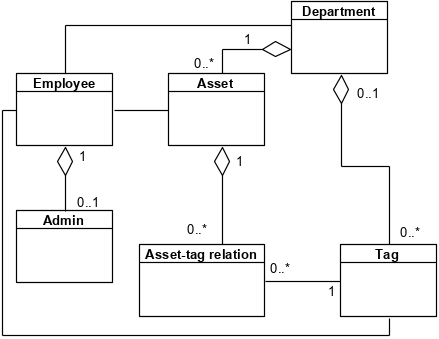
\includegraphics[width=0.8\textwidth]{figures/ClassDiagrams/Class_activity_class_diagram.png}
    \caption{Class diagram of the classes in the problem domain.}
    \label{fig:FirstPDClassDiagram}
\end{figure}

As described in \autoref{sc:classes}, there are six different relevant classes in the problem domain. These classes are: \textit{Employee}, \textit{Admin}, \textit{Department}, \textit{Asset}, \textit{Tag}, and \textit{Asset-tag relation}. The relations between these have been explained below.
\par

The \textit{Employee} class is an aggregation of the \textit{Admin} class. The structure created by this connection is a role pattern with only one role. The pattern makes it possible for an employee to possess the role of \textit{Admin} dynamically.
\par

The \textit{Asset} aggregates a number of \textit{Asset-tag relation}s. On top of this, every asset belongs to one department.
\par

The \textit{Employee} class has a association to the \textit{Asset}, \textit{Department}, and \textit{Tag} classes, as they can see the information on an asset and search for through them based on tags and/or departments. The \textit{Admin} class is a role of the \textit{Employee} class. This means that the functionality kept in the \textit{Admin} class will be available to the employees who have the role of admin.
\par

The \textit{Asset-tag relation} class is created to handle the relation between the \textit{Asset} and \textit{Tag} classes. The \textit{Asset} class aggregates it, as an asset the tags exists only as an addition to the assets. It has been added, as multiple assets can be tagged with the same tag and an asset can have multiple tags. The association to the \textit{Tag} class originates from the relation pattern. An instance of the \textit{Asset-tag relation} class always connects one asset and one tag, but both the \textit{Tag} and \textit{Asset} classes can be part of mulitple asset-tag relations.
\par

With the classes of the problem domain and their interconnecting relations described, the behaviour of the classes can be examined.

% Behavior activity
\section{Behavior} \label{sc:behavoir}
In the following section, the behavior of each class will be examined. A deeper understanding of these behaviours will be achieved through state chart diagrams.
\\\\

\large{\textbf{Asset}}
\begin{figure}[H]
    \centering
    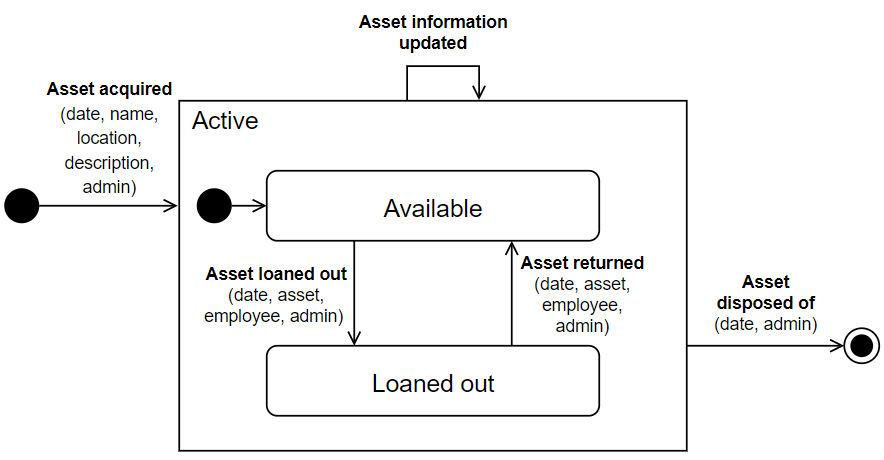
\includegraphics[width=1\textwidth]{figures/StateCharts/Asset_state_chart.png}
    \caption{State chart diagram for the \textbf{Asset} class}
    \label{fig:asset_statechart}
\end{figure}

An object of the \textit{Asset} class is created when an asset is acquired. At first, its state is \textbf{Available}, and when the asset is loaned out to an employee, it changes state to \textbf{Loaned out}. From any of these two states, the asset can be disposed of and removed from the problem domain. Being loaned out will, in the system, simply consist of the asset being tagged with an employee, and the return of the asset will be removing this relation. The information on the asset, not including the tags attached to it, can be updated at all times during its life cycle in the system, and can occur multiple times.
\\\\

\large{\textbf{Employee}}
\begin{figure}[H]
    \centering
    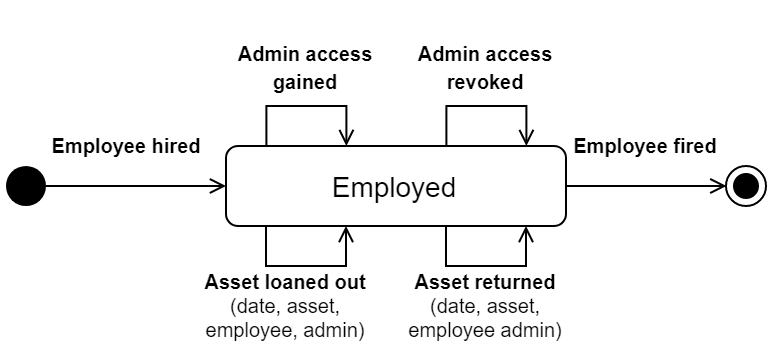
\includegraphics[width=0.8\textwidth]{figures/StateCharts/StateChart_Employee.png}
    \caption{State chart diagram for the \textbf{Employee} class}
    \label{fig:employee_statechart}
\end{figure}

An \textit{Employee} object is created when a person is hired at the zoo and gains the status employed. An employee can be granted admin access, which can later be revoked. An employee can also borrow an asset and return it later. The employee object ceases to exist when the person is fired. The event of returning an asset can only happen when the employee has borrowed the given asset, but an employee can borrow multiple assets at a time, hence both events are iterations.\\
The employee can be granted admin access multiple times during the employment but of course, the access can only be revoked after the access has been granted. Both things can happen multiple times and are therefore iterations. These two events also mark the initialization and end of an admin.
\\\\

\large{\textbf{Admin}}
\begin{figure}[H]
    \centering
    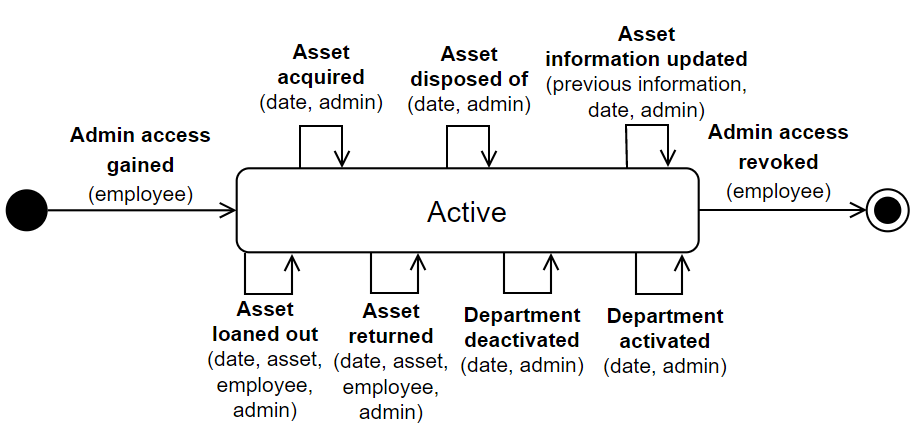
\includegraphics[width=0.8\textwidth]{figures/StateCharts/Admin_state_chart.png}
    \caption{State chart diagram for the \textbf{Admin} class}
    \label{fig:admin_statechart}
\end{figure}

The \textit{Admin} object is created when an employee is granted admin access. As an admin, the employee is responsible for loaning out assets to other employees and receiving the assets when they are returned. The admin will also be responsible for adding tags, assets, activating departments, and maintaining these elements by updating and removing them. The admin object is terminated when the employee's admin access is revoked.
\\\\

\large{\textbf{Tag}}
\begin{figure}[H]
    \centering
    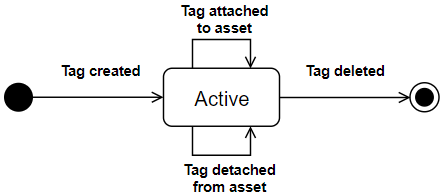
\includegraphics[width=0.6\textwidth]{figures/StateCharts/Tag_state_chart.png}
    \caption{State chart diagram for the \textbf{Tag} class}
    \label{fig:loan_statechart}
\end{figure}

An object of the \textit{Tag} class is created by an admin and can be attached to and detached from assets multiple times during its life cycle. The tag is terminated when an admin deletes it from the system.
\par

With the behaviours of the classes described, the problem domain has been analysed. The following section will sum up the results of the analysis.

% \large{\textbf{Loan}}
% \begin{figure}[H]
%     \centering
%     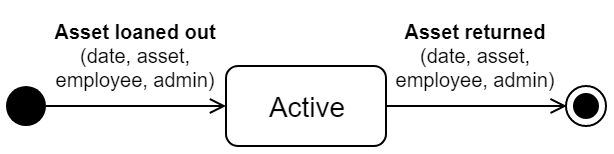
\includegraphics[width=0.8\textwidth]{figures/StateChart_Loan.png}
%     \caption{State chart diagram for the \textbf{Loan} class}
%     \label{fig:loan_statechart}
% \end{figure}

% A \textbf{Loan} object is created when an asset is loaned out and seizes to exist when the asset is returned.
% \newline\par
% With the behaviours of the classes described, the problem domain has been analysed. The following section will sum up the results of the analysis.

% Summary
\section{Summary} \label{ssc:pd_summary}
This chapter has discussed and analysed the different classes and events within the problem domain, as well as the structure and behavior of these. This has given an understanding of the interactions of the objects and an overview of the involved classes and events. The \textit{Tag} class has been added to the problem domain based on dialog with Aalborg Zoo, and the class has handled the loan of an asset to an employee, as well as improving the organizing of assets. The class diagram (see \autoref{fig:FirstPDClassDiagram}) depicts the classes that will form the core of the system and the connections between these. The event table (see \autoref{tab:events}) has listed all the initial events needed in the system to ensure the wanted functionality. Lastly the state charts of the classes (see \autoref{sc:behavoir}) have given an understanding of how the different classes behave and how they participate in different events.
\par

The overview, derived from these elements, has been used as a foundation for the system design and a better understanding of the application domain, which will be analysed in the following chapter..\\


%%%%%%%%%%%%%%%%%%%%%%%%%%%%%%%%%%%%%%%%%%%%%%%%%%%%%%%%%%%%%%%
% Application Domain Analysis
%%%%%%%%%%%%%%%%%%%%%%%%%%%%%%%%%%%%%%%%%%%%%%%%%%%%%%%%%%%%%%%
\chapter{Application Domain Analysis} \label{ch:applicationdomain}
In this chapter, the application domain has been analysed. This analysis involves the different actors, whom the system will be designed to interact with, and the different use cases these actors will go through as they use the system. The use cases have been constructed based on the requirements and the system definition, and make up a basis for the design of the interface and functionality of the system. Based on these, a functions list has been constructed.
\par
To sufficiently describe the needed functionality of the system, the usage of the system has been analysed. This description will be used to facilitate the design of the system and to ensure that it accommodates the way the actors will interact with it.

% Usage activity
\section{Usage}\label{sc:usage}
Within this section, the usage of the system, which include a list of actors and relevant use cases, has been analysed. This part of the application domain is important to understand, in order to create a satisfactory user experience and offer all the relevant functionality in the finished system. Firstly, the actors and use cases have been identified, described, and connected in an actor table.
\subsection{Actors} \label{scc:actors}
The actors in the application domain include the employees and admins. The differentiation of the two is made, because the admin has access to specific functionality and pages within the system, which are not available to the employee. As mentioned in the previous chapter, the admin is a role which an employee can take. This means that an admin has the same abilities as the employee as well as the extra functionalities the role provides.
\par
The descriptions of the actors include their level of experience with similar systems, their goals for using the system, and examples of the actor.

\fancyLayout{actor}{Admin}
    {Specification of the \textit{admin} actor.}
    {actor:admin}
    {
        \textbf{Goal:} The \textit{admin} manages the system. The \textit{admin's} basic goal is to keep track of the company assets.
        \vskip 0.2cm
        
        \textbf{Characteristics:} The \textit{admin} is the primary user of the system and is the only actor who can change anything regarding the assets in the system. They are experienced with using enterprise systems and handling the assets of their department.
        \vskip 0.2cm
        
        \textbf{Example:} This \textit{admin} is used to organising large quantities of assets, and sees the asset management system as a supplement to their organisational tools.
    }

The admin is, as mentioned, the primary user of the system and accommodating their needs has been of highest importance, when it comes to accommodating actor needs.

\fancyLayout{actor}{Employee}
    {Specification of the \textit{employee} actor.}
    {actor:employee}
    {
        \textbf{Goal:} The \textit{Employee} can borrow the company assets. They have a need for borrowing assets that are relevant to their work.
        \vskip 0.2cm
        
        \textbf{Characteristics:} The \textit{Employee} is the secondary user of the system. They can only borrow and view assets within the system. They have varying degrees of technical competence.
        \vskip 0.2cm
        
        \textbf{Examples:} \textit{Employee A} is familiar with computer systems and has no trouble finding their way around the asset management system.
        \vskip 0.1cm
        \textit{Employee B} is less experienced with computer systems and is more comfortable talking directly to the admin instead of using the system themselves. 
    }
As a secondary user of the system, the needs of the employee will have less priority than the needs of the admin.
\subsection{Use cases}\label{ssc:usecases}
The following use cases have been derived from the understanding of the problem domain and actors described in the previous sections. The following description of the use cases include how the interactions with the system will take place, which actors are involved, and which functions are called within the system to complete the actions.
\par
In addition to the already described interactions stated in the system definition, the interviews with Aalborg Zoo have let to the use case of an admin printing out a report of assets from the system. The report can consist of all or some of the assets in the system and will be saved as a separate file on the admins computer.
% \par
% Each use case has been described and is followed by a diagram of the interaction.
\newline

\fancyLayout{use_case}{Add an asset}
    {Use case for adding an asset}
    {use_case:add_an_asset}
    {
        \textbf{Use Case:} Adding an asset is done by an admin. The admin goes to the add asset page, attaches the relevant tags, and fills in the relevant information about the asset. The admin then saves the asset in the system and it becomes visible to all employees.
    
        \vskip 0.2cm
        
        \textbf{Objects:} Admin, Asset
        
        \vskip 0.2cm
        
        \textbf{Functions:} Add asset
    }

\begin{figure}[H]
    \centering
    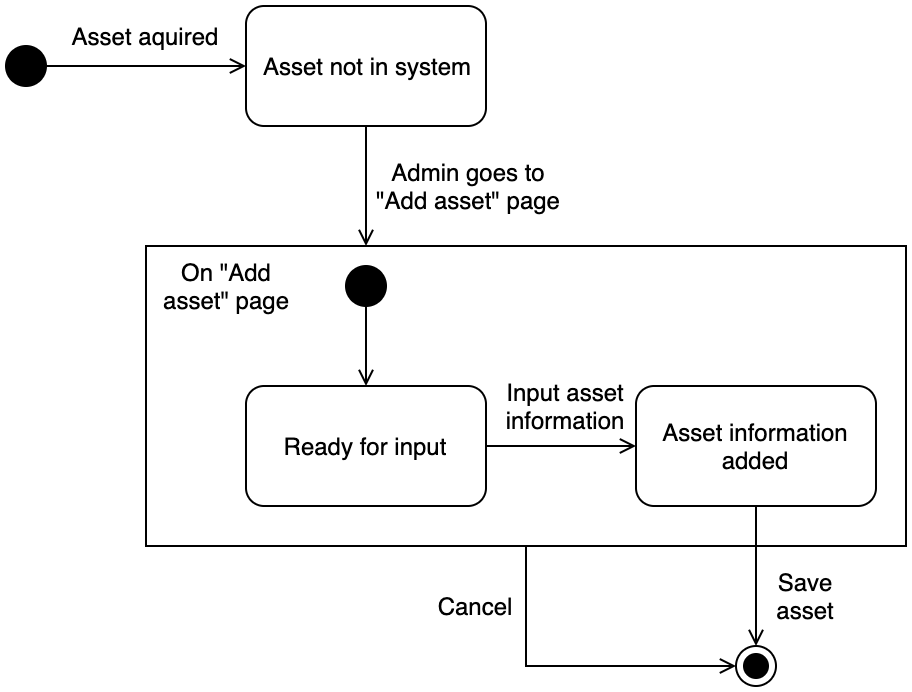
\includegraphics[width=0.8\textwidth]{figures/UseCases/UC_Add_asset.png}
    \caption{User interface state chart diagram for adding an asset}
    \label{fig:add_asset_statechart}
\end{figure}

\newpage

\fancyLayout{use_case}{Loan out an asset}
    {Use case for loaning out an asset}
    {use_case:loan_out_an_asset}
    {
        \textbf{Use Case:} Loaning out an asset is done by an admin, whom an employee contacts, when they want to borrow the given asset. The admin goes to the page of the given asset and attaches the employee's tag to it. The admin then hands over the asset to the employee.
    
        \vskip 0.2cm
        
        \textbf{Objects:} Admin, Asset, Employee, Tag
        
        \vskip 0.2cm
        
        \textbf{Functions:} Asset loaned out, Tag attached to asset
    }
 
\begin{figure}[H]
    \centering
    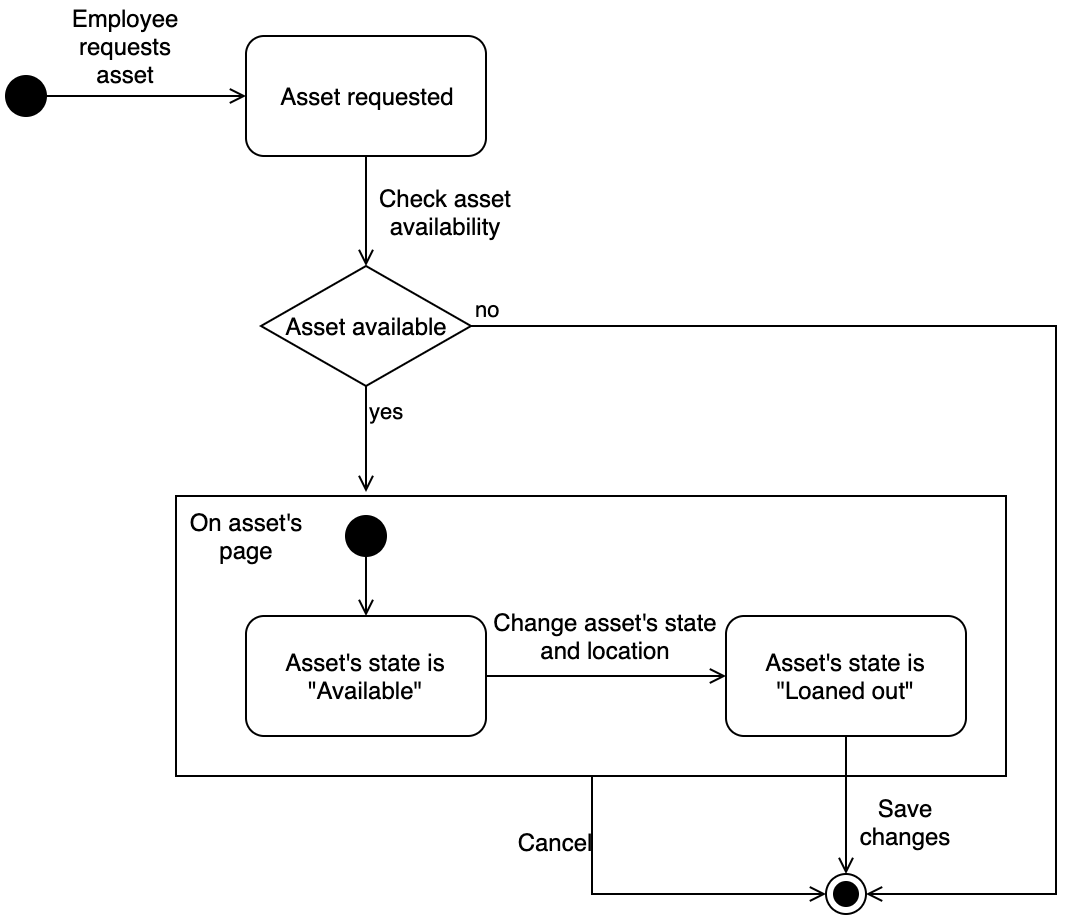
\includegraphics[width=0.8\textwidth]{figures/UseCases/UC_Loan_out_asset.png}
    \caption{User interface state chart diagram for loaning out an asset}
    \label{fig:loan_out_asse_statechart}
\end{figure}
\todo{Update diagram}
 
\fancyLayout{use_case}{Return an asset}
    {Use case for returning an asset}
    {use_case:return_an_asset}
    {
        \textbf{Use Case:} When an asset is being returned by an employee, it is handed over to an admin. The admin then goes to the page of the given asset and detaches the tag of the employee from the asset.
    
        \vskip 0.2cm
        
        \textbf{Objects:} Admin, Asset, Employee, Tag
        
        \vskip 0.2cm
        
        \textbf{Functions:} Update asset information, Tag detached from asset
    }
    
\begin{figure}[H]
    \centering
    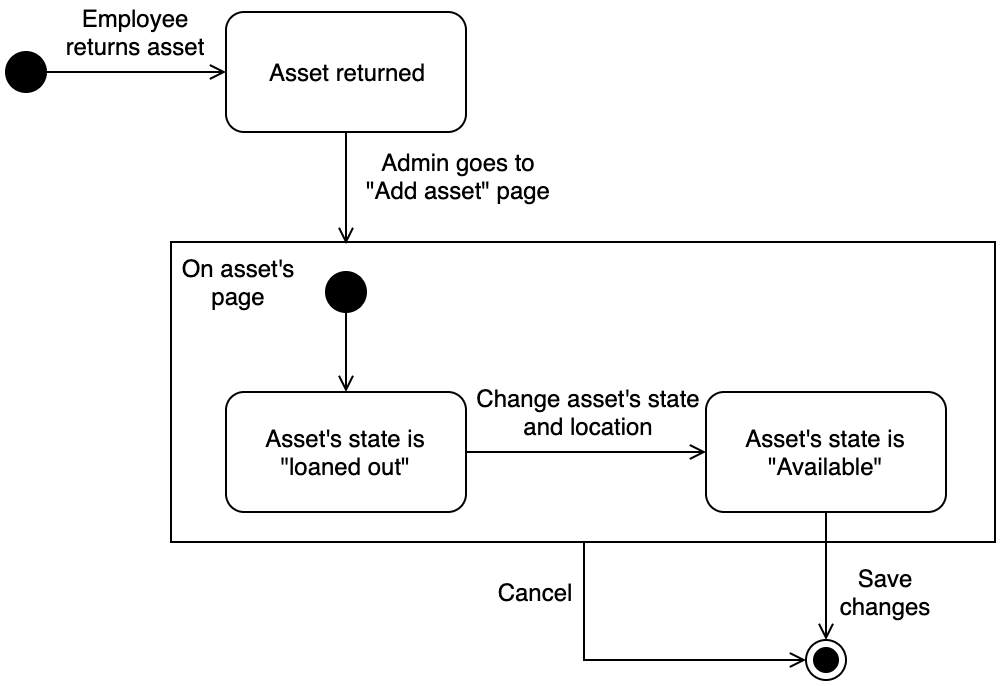
\includegraphics[width=0.8\textwidth]{figures/UseCases/UC_Return_asset.png}
    \caption{User interface state chart diagram for returning an asset}
    \label{fig:return_asset_statechart}
\end{figure}
\todo[inline]{Update diagram}

\fancyLayout{use_case}{Change the information of an asset}
    {Use case for changing the information of an asset}
    {use_case:changing_the_information_about_an_asset}
    {
        \textbf{Use Case:} If one of the states of an asset changes, the changed data should be updated in the system by an admin. These changes could be things such as the asset going from working to being broken or being updated to a new operation system. To update the asset's information, the admin goes to the given asset's page, can then press the edit button, and change the outdated data to comply with the new state of the asset in the problem domain.
    
        \vskip 0.2cm
        
        \textbf{Objects:} Admin, Asset
        
        \vskip 0.2cm
        
        \textbf{Functions:} Search for asset, Update asset information, View asset
    }
    
\begin{figure}[H]
    \centering
    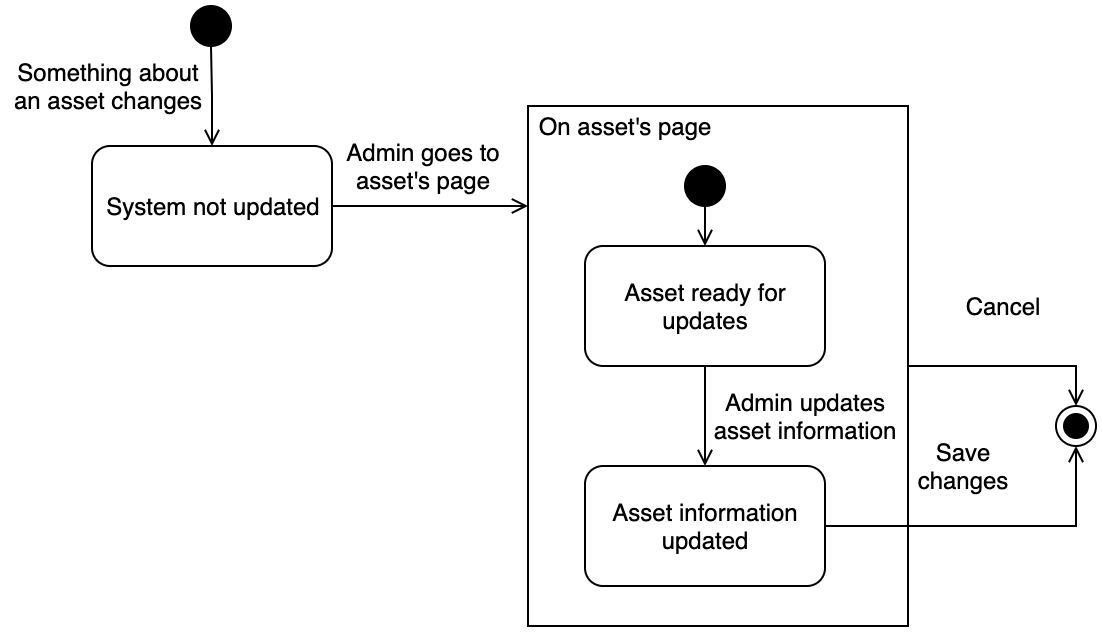
\includegraphics[width=0.8\textwidth]{figures/UseCases/UC_Change_asset.png}
    \caption{User interface state chart diagram for changing an asset}
    \label{fig:edit_asset_statechart}
\end{figure}

\newpage

\fancyLayout{use_case}{Remove an asset}
    {Use case for removing an asset}
    {use_case:remove_an_asset}
    {
        \textbf{Use Case:} When an asset is no longer needed within the problem domain, it is discarded. This is handled in the system by an admin. The admin goes to the page of the given asset and deletes it from the system. The asset is then removed from the system and is no longer visible to any of the employees.
    
        \vskip 0.2cm
        
        \textbf{Objects:} Admin, Asset, Employee
        
        \vskip 0.2cm
        
        \textbf{Functions:} Remove asset
    }

\begin{figure}[H]
    \centering
    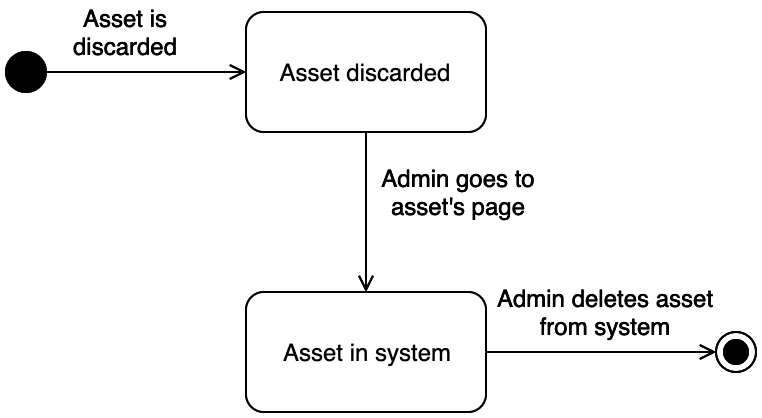
\includegraphics[width=0.8\textwidth]{figures/UseCases/UC_Remove_asset.png}
    \caption{User interface state chart diagram for removing an asset}
    \label{fig:remove_asset_statechart}
\end{figure}

\newpage

\fancyLayout{use_case}{Search for an asset}
    {Use case for searching for an asset}
    {use_case:search_for_an_asset}
    {
        \textbf{Use Case:} If a user wants information about a specific asset, this can be achieved by going to the search page and entering some information about the asset in the search field. The system then returns a list of assets complying with the search query. The user can then choose the desired asset.
    
        \vskip 0.2cm
        
        \textbf{Objects:} Admin, Asset, Employee
        
        \vskip 0.2cm
        
        \textbf{Functions:} Search for asset, View asset
    }

\begin{figure}[H]
    \centering
    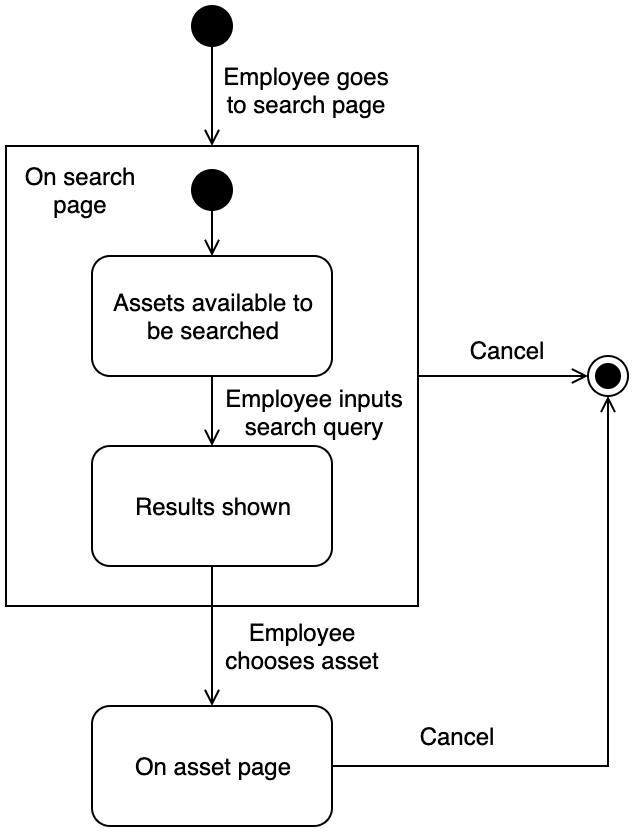
\includegraphics[width=0.6\textwidth]{figures/UseCases/UC_Search_asset.png}
    \caption{User interface state chart diagram for searching for an asset}
    \label{fig:search_asset_statechart}
\end{figure}

\fancyLayout{use_case}{Print a report of assets}
    {Use case for printing a report of assets}
    {use_case:print_a_report_of_assets}
    {
        \textbf{Use Case:} As the number of assets in the system increases, an admin might want to retrieve a number of assets from the system. The admin goes to the asset list page, selects the assets they want to retrieve from the system and presses the print button. The system then generates a file containing information about the selected assets and saves it on the admin's computer.
    
        \vskip 0.2cm
        
        \textbf{Objects:} Admin, Asset
        
        \vskip 0.2cm
        
        \textbf{Functions:} Export report
    }

\begin{figure}[H]
    \centering
    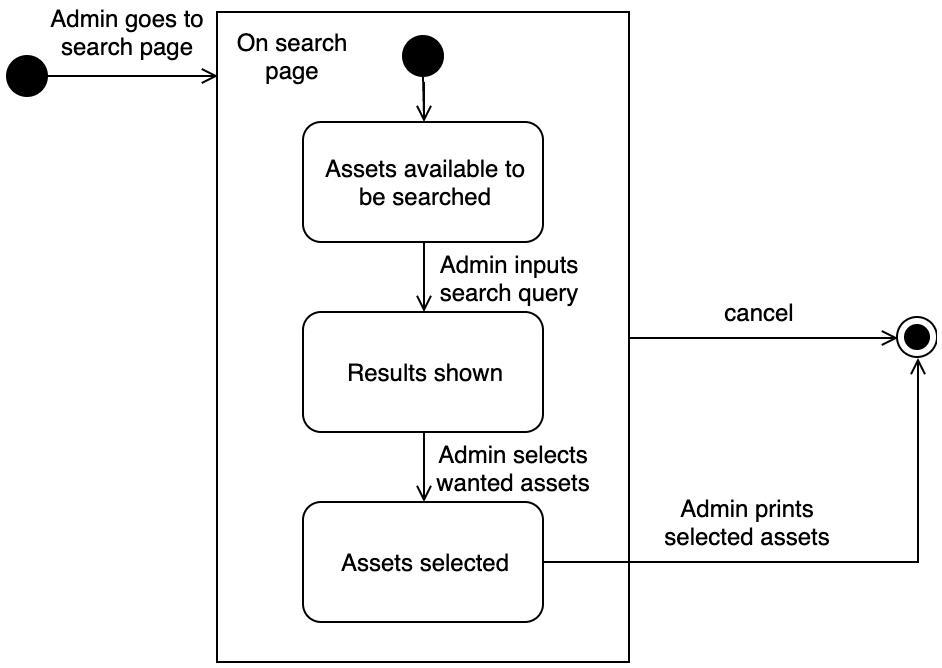
\includegraphics[width=0.8\textwidth]{figures/UseCases/UC_Print_report.png}
    \caption{User interface state chart diagram for printing out a report}
    \label{fig:print_report_statechart}
\end{figure}

\fancyLayout{use_case}{Comment on an asset}
    {Use case for commenting on an asset}
    {use_case:commenting_on_an_asset}
    {
        \textbf{Use Case:} A user might have a comment regarding an asset, such as an issue they have had with it or suggestions for improvements. To share this information with other users, they can go to the page of the asset and add a comment to it. This comment will be visible to all users.
    
        \vskip 0.2cm
        
        \textbf{Objects:} Admin, Asset, Employee
        
        \vskip 0.2cm
        
        \textbf{Functions:} Add comment to asset, Search for asset, View Asset
    }

\begin{figure}[H]
    \centering
    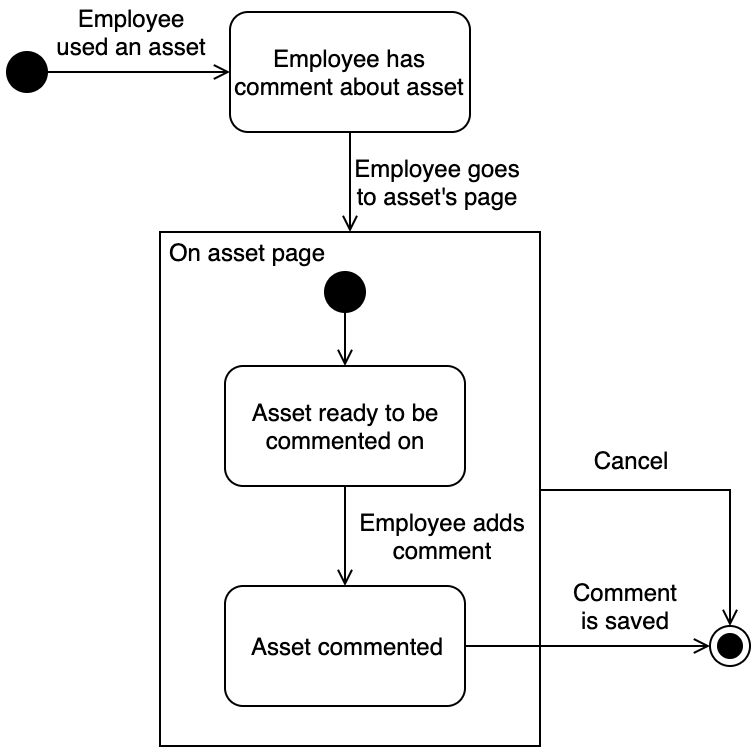
\includegraphics[width=0.8\textwidth]{figures/UseCases/UC_Add_comment.png}
    \caption{User interface state chart diagram for adding a comment to an asset}
    \label{fig:add_comment_statechart}
\end{figure}

These are the relevant use cases for managing the assets. The use cases have been placed in an actor table with the two previously described actors in order to illustrate the connections between these.

\begin{table}[H]
    \centering
    % \hrule
    \vspace{0.2cm}
    \hspace{6cm} \vspace{0.6cm} \textbf{Actors}
    \begin{tabular}{p{0.5\textwidth} || p{0.2\textwidth} p{0.2\textwidth}}
        \textbf{Use cases} & Admin & Employee \vspace{0.2cm}\\
        \hline \hline
        Add an asset & \hspace{0.34cm} \checkmark & \\
        \hline
        Loan out an asset & \hspace{0.34cm} \checkmark & \hspace{0.6cm} \checkmark \\
        \hline
        Return an asset & \hspace{0.34cm} \checkmark & \hspace{0.6cm} \checkmark \\
        \hline
        Change the information about an asset & \hspace{0.34cm} \checkmark & \\
        \hline
        Remove an asset & \hspace{0.34cm} \checkmark & \\
        \hline
        Search for an asset & \hspace{0.34cm} \checkmark & \hspace{0.6cm} \checkmark \\
        \hline
        Print a report of assets & \hspace{0.34cm} \checkmark & \\
        \hline
        Comment an asset & \hspace{0.34cm} \checkmark & \hspace{0.6cm} \checkmark\\
    \end{tabular}
    \vspace{0.2cm}
    % \hrule
    \vspace{0.2cm}
    \caption{Actor table of the relations between actors and use cases.}
    \label{tab:actor_table}
\end{table}

As the actor table above shows, the admin takes part in every use case. This can be explained by the way the system will be used. The system should function almost like an interface to a database, so it makes sense that the admin will be involved in all the changes made to the system and the database.\\

The defined use cases have then been used to extract relevant functions and, later in the report, construct the user interface (see \autoref{ch:ui_design}). For most of these use cases, the system should limit the access of the employees without admin status, which has resulted in two additional functions, \textit{Authenticate user} and \textit{Check access level}. These functions are used to guarantee that parts of the system is only accessible to employees with admin status and are executed on login and most of the described use cases above.
\par
The functions discovered in this section have been analysed and described in the following section.

% Function activity
\section{Function activity}\label{sc:function}
Based on the use cases, it is possible to determine the functions necessary for the system to adequately fulfill the requirements. These functions have been classified by their type and complexity in the following function list. The complex functions have then been further split into smaller functions to explain their processes. This is done following the functions analysis and the complexity definitions from \cite[chap 7]{OOAD}. The complexity definitions are:
\begin{itemize}
    \item Simple: Sets or reads the value of an attribute in an existing object.
    \item Medium: Creates a new object and connects it by object structure(s) to other objects.
    \item Complex: Reads from or creates several objects (from different classes).
\end{itemize}
With these definitions, the following function table has been constructed.

\begin{table}[H]
\centering
    \begin{tabular}{|l|l|l|}
        \hline
        \textbf{Function} & \textbf{Complexity} & \textbf{Type} \\
        \hline
        \hline
        Add asset & Complex & Update\\
        \hline
        Remove asset & Simple & Update\\
        \hline
        Update asset information & Complex & Update\\
        \hline
        Comment asset & Medium & Update\\
        \hline
        Search for asset & Medium & Compute/Read\\
        \hline
        View asset & Simple & Read\\
        \hline
        Add department & Simple & Update\\
        \hline
        Remove department & Simple & Update\\
        \hline
        Authenticate user & Simple & Read\\
        \hline
        Check access level & Simple & Read\\
        \hline
        Export report & Complex & Compute/Read\\
        \hline
        Attach tag & Simple & Update\\
        \hline
        Detach tag & Simple & Update\\
        \hline
    \end{tabular}
\caption{Function table showing all the different top-level functions as well as their complexity and type.}\label{tab:functions}
\end{table}

The function table (see \autoref{tab:functions}) contains multiple complex functions. As mentioned earlier, these functions have been further split into smaller functions to better understand the operations.


\fancyLayout
    {function}
    {Add asset}
    {The table shows the different functions involved in adding an asset as well as their complexity.}
    {function:add_asset}
    {
        \centering
        \begin{tabular}{|l|l|l|}
            \hline
            \textbf{Function} & \textbf{Complexity} & \textbf{Type}\\
            \hline
            \hline
            Add relevant information about the asset & Simple & Update \\
            \hline
            Save Asset to model & Medium & Update \\
            \hline
            Update connections to tags & Medium & Update\\
            \hline
        \end{tabular}
}

The \textit{Add asset} function consists of three smaller functions, as seen in \autoref{function:add_asset}. When adding an asset, first the admin enters the relevant information, which is then saved with the asset to the model. Lastly, the \textit{Asset-tag relation}s connected to the asset are updated. This last step possibly creates and deletes \textit{Asset-tag relation}s between the asset and the relevant tags.

\fancyLayout
    {function}
    {Update asset information}
    {The table shows the different functions involved in updating an assets information.}
    {function:update_asset_information}
    {
        \centering
        \begin{tabular}{|l|l|l|}
            \hline
            \textbf{Function} & \textbf{Complexity} & \textbf{Type}\\
            \hline
            \hline
            Load asset from model & Simple & Read \\
            \hline
            Update relevant information about the asset & Simple & Update \\
            \hline
            Save asset to model & Medium & Update \\
            \hline
            Update connections to tags & Medium & Update\\
            \hline
        \end{tabular}
}

The \textit{update asset information} function is made up of the smaller functions, as shown in \autoref{function:update_asset_information}, which will be executed in the shown order. First, the asset is loaded from the model and formatted as an asset in the system. Then the changes to the information is applied to the asset. The asset is then saved to the model with the changes and its connections to tags are updated. Just as the \textit{Add asset} function, the last step possibly creates and deletes \textit{Asset-tag relation}s between the asset and the relevant tags.

\fancyLayout
    {function}
    {Export report}
    {The table shows the different functions involved in exporting a report.}
    {function:export_report}
    {
        \centering
        \begin{tabular}{|l|l|l|}
            \hline
            \textbf{Function} & \textbf{Complexity} & \textbf{Type}\\
            \hline
            \hline
            Load assets to be included & Simple & Update \\
            \hline
            Create entries & Simple & Update \\
            \hline
            Build report & Simple & Update \\
            \hline
            Export to CSV-format & Medium & Compute \\
            \hline
        \end{tabular}
}

The \textit{export report} function involves the four smaller functions listed in \autoref{function:export_report}, happening in order. The first step is that the selected assets are loaded. Then report entries are created based on the assets, which are then added to the report. Finally the report is exported to the admin's computer formatted as a Comma Separated Values (CSV) file.
\par
This concludes the analysis of functions. The understanding of the users and functions has been used in the following section as a basis for the interface.
\section{Functions}\label{sc:functions}

This section will present the functions in the system. Table \ref{tab:functions} shows all the top-level functions that the system will be able to perform. All the tables describing functions have columns with the name of the function, the complexity and the type of function.

\begin{table}[H]
\centering
%\resizebox{\textwidth}{!}{%
    \begin{tabular}{|l|l|l|}
        \hline
        \textbf{Function} & \textbf{Complexity} & \textbf{Type} \\
        \hline
        \hline
        Add asset & Complex & Update\\
        \hline
        Remove asset & Medium & Update\\
        \hline
        Edit asset & Complex & Update\\
        \hline
        Search asset & Medium & Compute/Read\\
        \hline
        View asset & Simple & Read\\
        \hline
        Add tag & Simple & Update\\
        \hline
        Remove tag & Medium & Update\\
        \hline
        Rename tag & Simple & Update\\
        \hline
        Tag asset & Simple & Update\\
        \hline
        Untag asset & Simple & Update\\
        \hline
        Authenticate user & Simple & Read\\
        \hline
        Check access level & Simple & Read\\
        \hline
        Export report & Complex & Compute/Read\\
        \hline
        Export log & Complex & Compute/Read\\
        \hline
    
    \end{tabular}
%}
\caption{Table showing all the different top-level functions as well as their complexity and type.}\label{tab:functions}
\end{table}

\par

Table \ref{tab:functions} contains several functions rated complex. These functions have been divided into several smaller functions, with a lower complexity.
% Beskriver hvorfor det er gjort, ved ikke om det skal med, men det er god fyldertekst
This is done in order to divide the complex problems into smaller problems, which are easier to implement. 
 
\begin{center}
    \textbf{Adding an asset}
\end{center}

% Add asset table
\begin{table}[H]
\centering
%\resizebox{\textwidth}{!}
\caption{Table showing the different functions involved in adding an asset along with their complexity and type.}\label{tab:AddAssetFunctions}
\end{table}

\par

\begin{center}
    \textbf{Editing an asset}
\end{center}

% Edit Asset Table
\begin{table}[H]
\centering
%\resizebox{\textwidth}{!}
\caption{Table showing the different functions involved in editing an asset along with their complexity and type.}\label{tab:EditAssetFunctions}
\end{table}

\par

% \begin{center}
%     \textbf{Adding a template}
% \end{center}

% % Add template table 
% \begin{table}[H]
% \centering
% %\resizebox{\textwidth}{!}{%
%     \begin{tabular}{|l|l|l|}
%         \hline
%         \textbf{Function} & \textbf{Complexity} & \textbf{Type} \\
%         \hline
%         \hline
%         Add Field & Simple & Update\\
%         \hline
%         Save Template & Medium & Update\\
%         \hline
        
%     \end{tabular}
% %}
% \caption{Table showing the different functions involved in adding a template along with their complexity and type.}\label{tab:AddTemplateFunctions}
% \end{table}

% \par

% \begin{center}
%     \textbf{Editing a template}
% \end{center}

% % Edit template table
% \begin{table}[H]
% \centering
% %\resizebox{\textwidth}{!}{%
%     \begin{tabular}{|l|l|l|}
%         \hline
%         \textbf{Function} & \textbf{Complexity} & \textbf{Type} \\
%         \hline
%         \hline
%         Add Field & Simple & Update\\
%         \hline
%         Remove Field & Simple & Update\\
%         \hline
%         Load Template & Medium & Read\\
%         \hline
%         Save Template & Medium & Update\\
%         \hline
        
%     \end{tabular}
% %}
% \caption{Table showing the different functions involved in editing a template along with their complexity and type.}\label{tab:EditTemplateFunctions}
% \end{table}

% \par

\begin{center}
    \textbf{Exporting a report}
\end{center}

% Export report table
\begin{table}[H]
\centering
%\resizebox{\textwidth}{!}
\caption{Table showing the different functions involved in exporting a report along with their complexity and type.}\label{tab:ExportReportFunctions}
\end{table}

% User interface
\section{User interface}\label{sc:userinterface}
% intro intro

\begin{figure}[H]
    \centering
    \frame{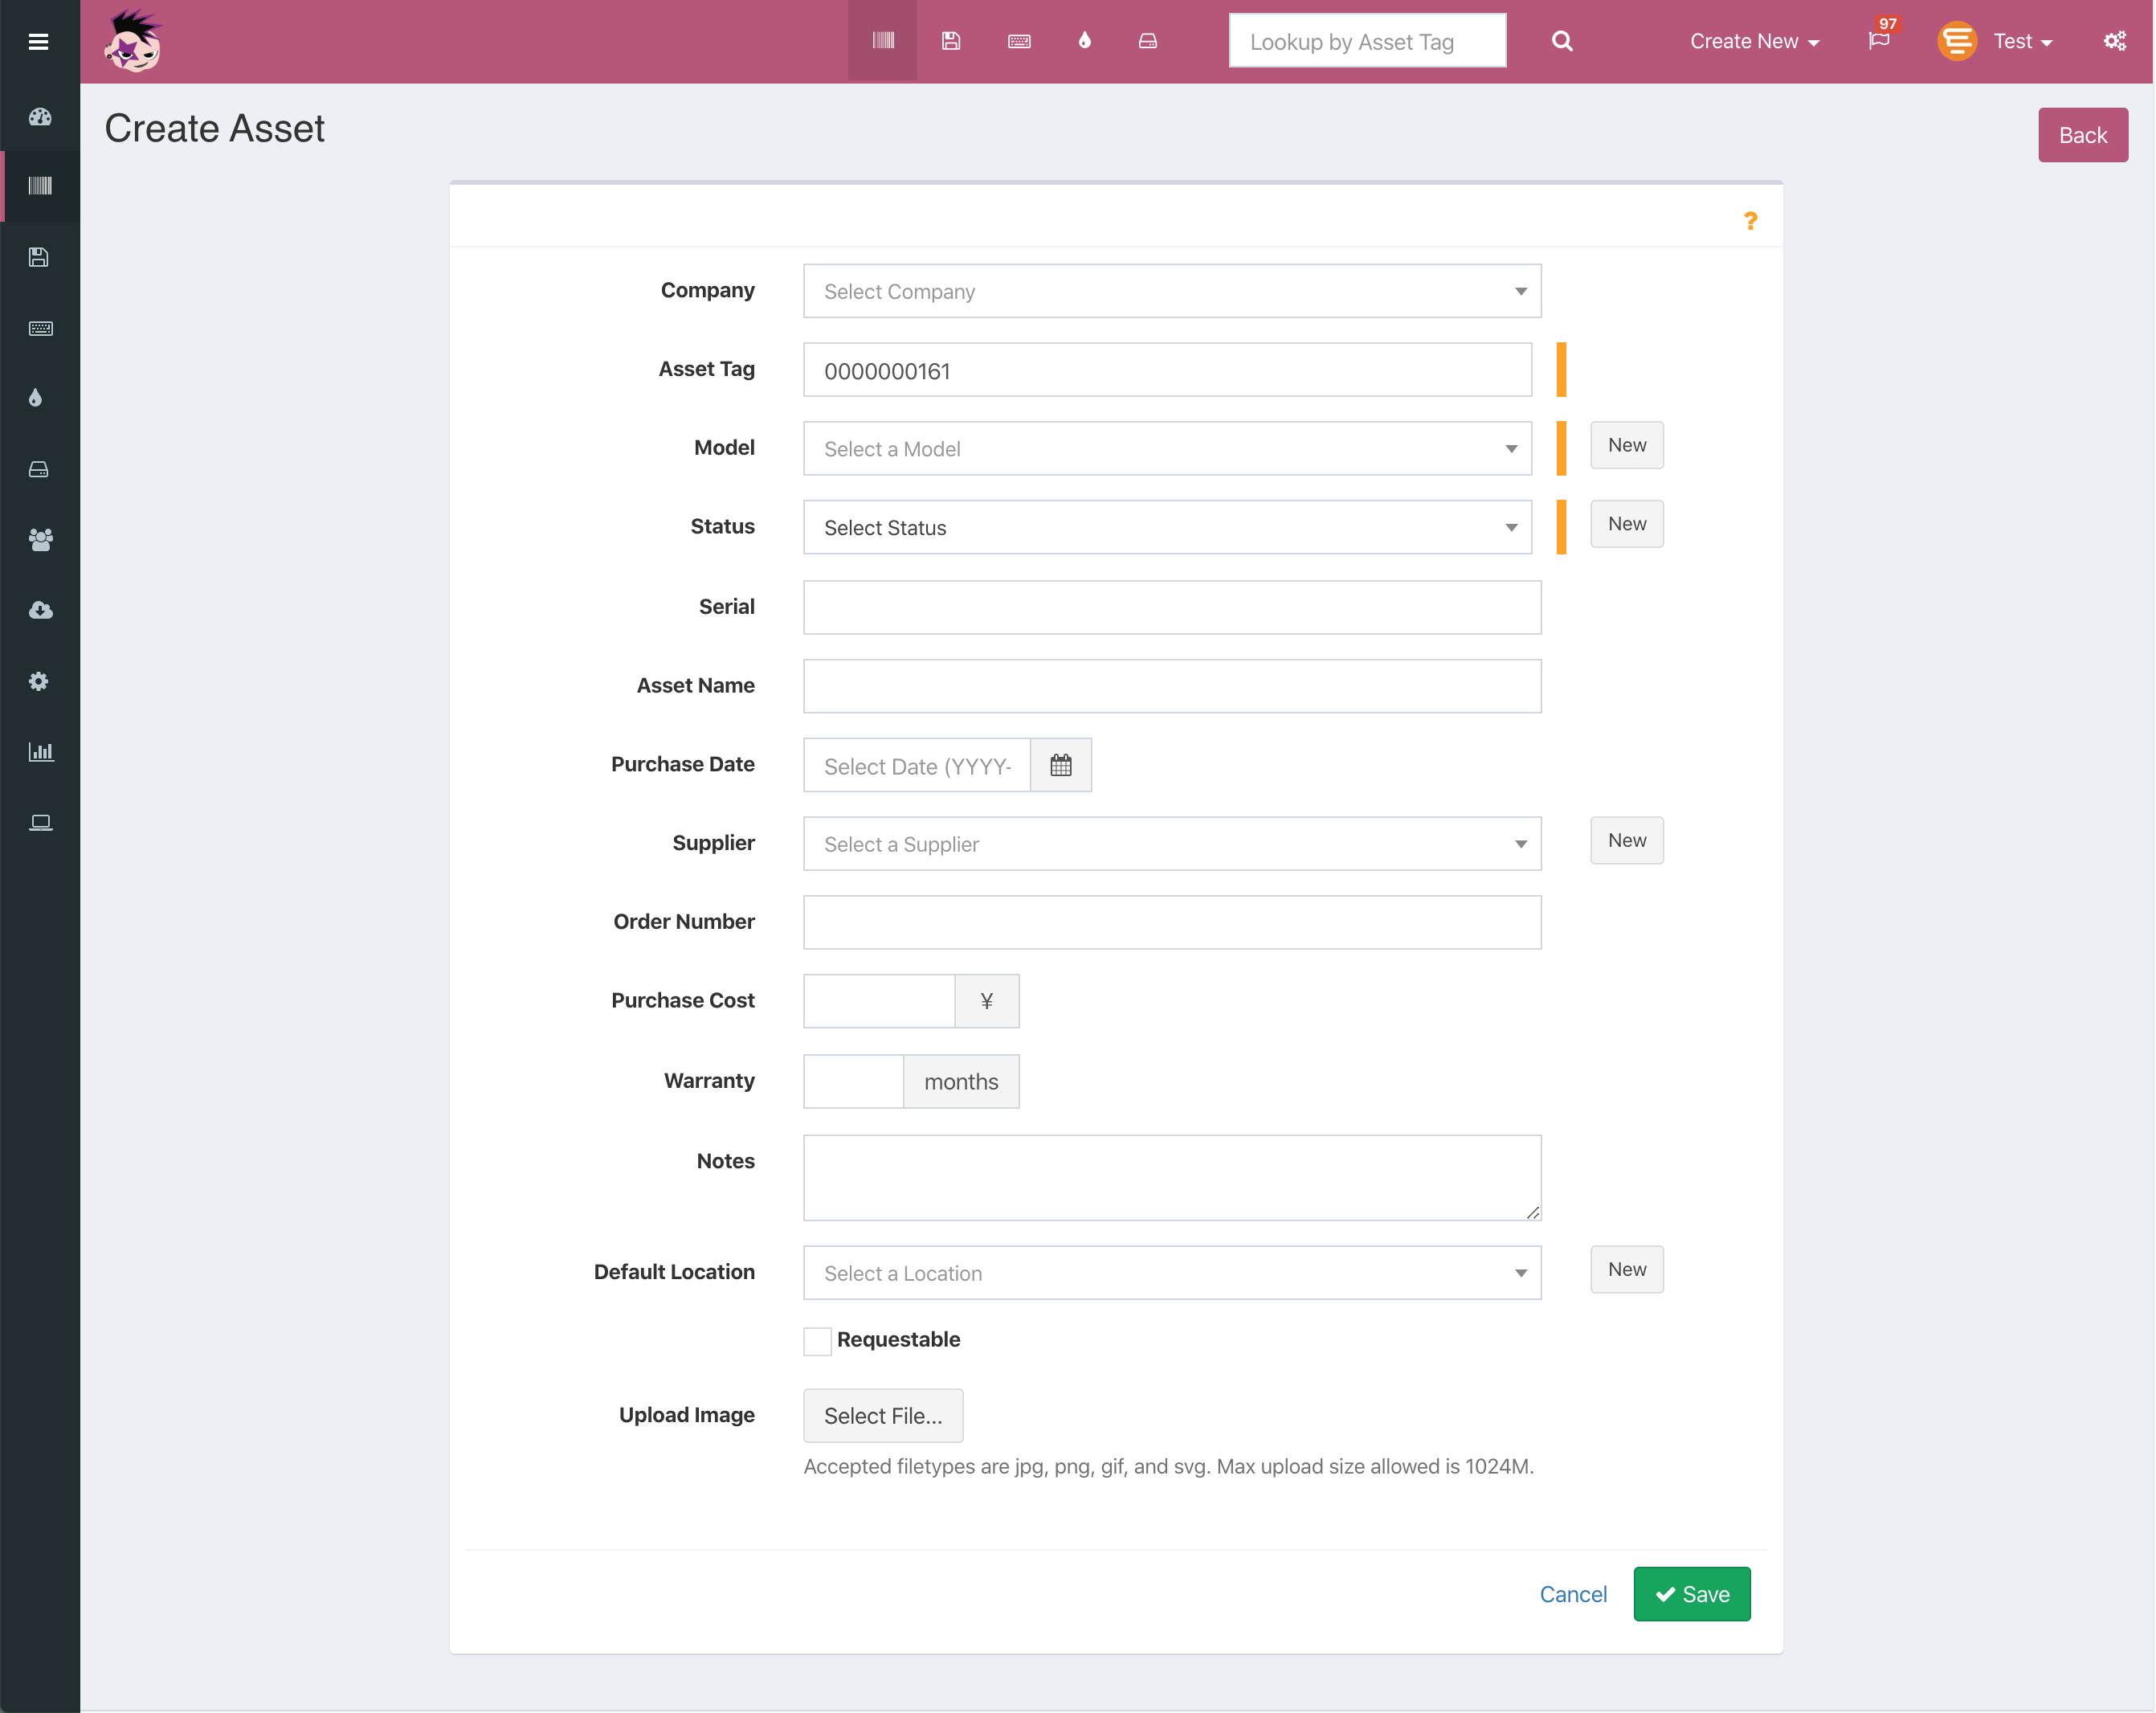
\includegraphics[width=0.9\textwidth]{figures/other-systems/snipeitapp-create-asset-ui-screenshot.png}}
    \caption{Caption}
    \label{fig:too}
\end{figure}


The user interface is following the KISS-principle (Keep It Simple Stupid) and therefore only contains the utmost required interface-elements. As mentioned in \autoref{ch:introduction} and \autoref{ch:problemdefinition} our client needs an easier process of maintaining assets compared to existing solutions on the market. Existing solutions often present the user with a number of fields depending on the category an asset belongs to. This often result in empty and unnecessary fields that are never used. Our approach is based on fields dynamically appearing based on tags added to an asset.

\begin{figure}[H]
    \centering
    \frame{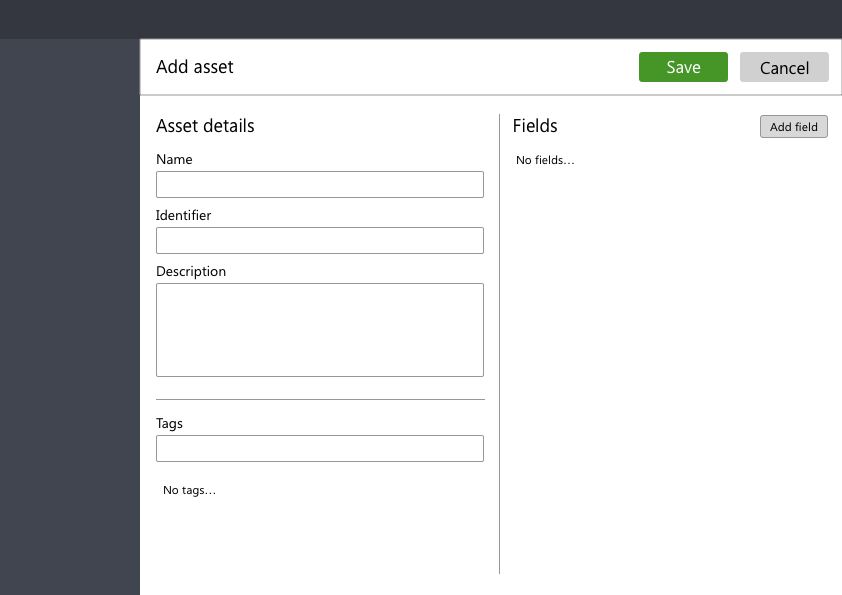
\includegraphics[width=0.9\textwidth]{figures/wireframes/add-asset-no-tags.png}}
    \caption{The process of creating a new asset, at this point no tags or custom fields were added, resulting in no fields beside base fields.}
    \label{fig:add-asset-no-tags}
\end{figure}

\begin{figure}[H]
    \centering
    \frame{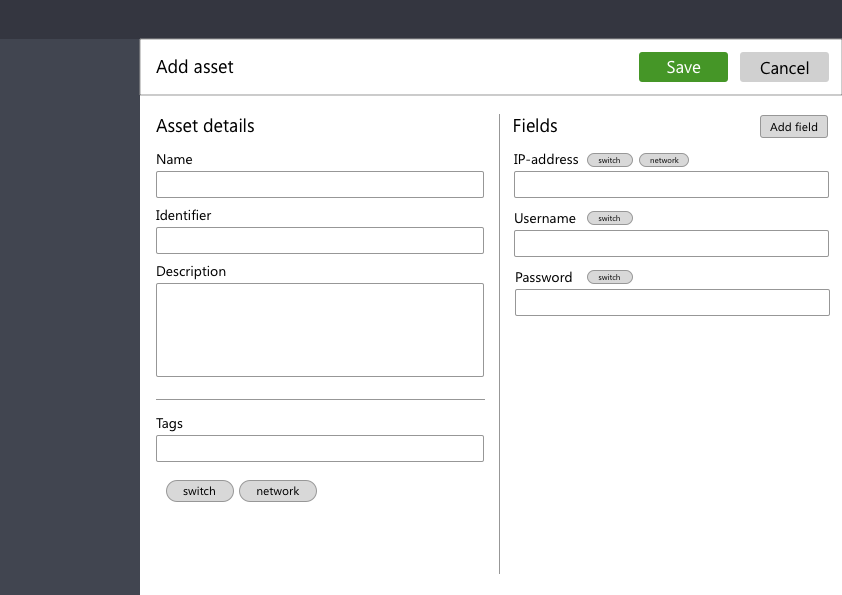
\includegraphics[width=0.9\textwidth]{figures/wireframes/add-asset-with-tags.png}}
    \caption{User interface state chart diagram for searching for an asset}
    \label{fig:add_asset_with_tags}
\end{figure}


\subsection{Employee}
Employees have access to the application and are capable of performing basic operations within the system.

\textbf{Splashscreen:} the first screen visible to the user at application startup 

% Dash / overview page
% Assets list page
% Asset view
% Add comments to asset
% Edit/remove own assets
% Menues?

\subsection{Admin}
Admins are able to do everything an Employee can but their enhanced access make them able to manage system content.

% Add/edit/delete departments
% Add/edit/delete assets
% Add/edit/delete tags
% Add/edit/delete all comments
% Read logs
% Export reports
% Import user data from third-part // Allowing employees access to the system
% 
\subsection{PACT analysis}\label{ssc:PACT}
A PACT analysis \cite[chap 2]{DEB} has been performed to better understand the interactions between the users and the system. The analysis gives a better description of the users, their needs and restrictions, the context in which the system is used, the activities surrounding the system, and the technologies involved.\\

\textbf{People}:\\
%(Physiological differences, Psychological differences, Social differences, Domain Expertise)
It is important to analyse the interactions with the system, to ensure ease of use for the people using the system. It should be taken into consideration, how these people are different from each other and what special needs they might have. First we list the people who will interact with the system:

\begin{itemize}
    \setlength\itemsep{0.05em}
    \item Admins at the zoo (primarily at the IT department)
    \item Employees at the zoo
\end{itemize}

The presented people have no psychological, physiological, or social differences to speak of. The respondents from the zoo, Morten and Kasper, both work in the IT department, which means they are used to working with computers. They are the main focus of the system, as they are the ones who will use it the most. However, they have requested the interface to be minimalistic and easy to use. The other employees at the zoo are expected to have experience with computer-based systems through their work, but not as deep of an understanding as Morten and Kasper. This information has been derived from the interviews with Morten and Kasper.\\

\textbf{Activities}: \\
%(Purpose of activities to be supported by the system, Temporal aspects, Collaboration, Complexity, Safety criticality, Nature of system content) \\
The users of the system will be using the system to keep track of assets and export lists of assets. They will keep track of the assets by adding them to, editing them in, and removing them from the system. They will also print out a list of changes made to the assets. On occasion they may also want a specific asset and will search through the database. Some users will only use the system to see assets and their state, and comment on them. The system will also be used to create groups of assets based on tags.\\

\textbf{Context}: \\
%(Physical, Social, Organizational) \\
The system will be used at Aalborg Zoo, primarily on desktops and laptops located within the zoo. The laptops might be moved around the premise. The social context at the zoo is not expected to be affected by the system, as it does not contain any elements geared towards any social aspects.\\
 
\textbf{Technology}:
%(That could support users in the domain)
The relevant technologies related to the system and its implementation include the following:

\begin{itemize}
    \setlength\itemsep{0.05em}
    \item Computer
    \item Screen
    \item Barcode scanner
    \item Mouse
    \item Keyboard
    \item Database
    \item Internet
\end{itemize}

The computer will be used to run the system and the screen will be used as an output device, while the barcode scanner, mouse, and keyboard will be used for input. The database will function as storage for everything added to the system, such as assets and tags, and the internet will be used in the context of connecting to the database and maintaining the model on all connected devices running the system.
\par
With a deeper understanding of the people, activities, contexts, and technologies surrounding the system, it is easier to design the user interface of the system.
\subsection{User interface}\label{ssc:UIAnalysis}
% goal and target users
The goal of the user interface is to provide an overview of the assets managed by the system, and enable the user to oversee them. The target users for this system are experienced in using computer programs. It is therefore not necessary to guide the user thoroughly through the systems functionalities.
\par

% supported activities and contexts. Short bursts of usage
Setting up the system and adding all the assets and relevant information will take time and effort on the users part. Afterwards, however, the user will only interact with the system in small bursts, when making small additions or deletions. There will not be an employee assigned to the system full time. Because of this, it is relevant to design the system in a way that allows the user to perform their tasks as fast as possible, and get on with their other work.
\par
As the work periods are short, user attention is less of an issue, since the user should be able to plan their work in the system to minimize external distractions. As the users work at an IT department, it is however possible for unpredictable interruptions to occur, when other employees might come by with questions or requests. As such, the system should be designed in a way that allows for the users attention to be divided, at least to a certain extent, without the user making major mistakes. This can be done by making it possible to save what is being worked on before it is completely done, so the user can return to finish it later. Making the system fast and responsive can also make it easier to handle distractions, as it will be easier to quickly finish the current task, despite potential interruptions. 
\par

% Hvordan vil vi designe UI'et?
The user interface should only contain the utmost required interface-elements. As mentioned in \autoref{ch:introduction} and \autoref{ch:problemdefinition}, the client needs an easier process for managing assets compared to existing solutions on the market. Existing solutions often present the user with a number of fields depending on the category an asset belongs to (see \autoref{fig:too-many-fields}). This often results in empty and unnecessary fields that are never used. 

\begin{figure}[H]
    \centering
    \frame{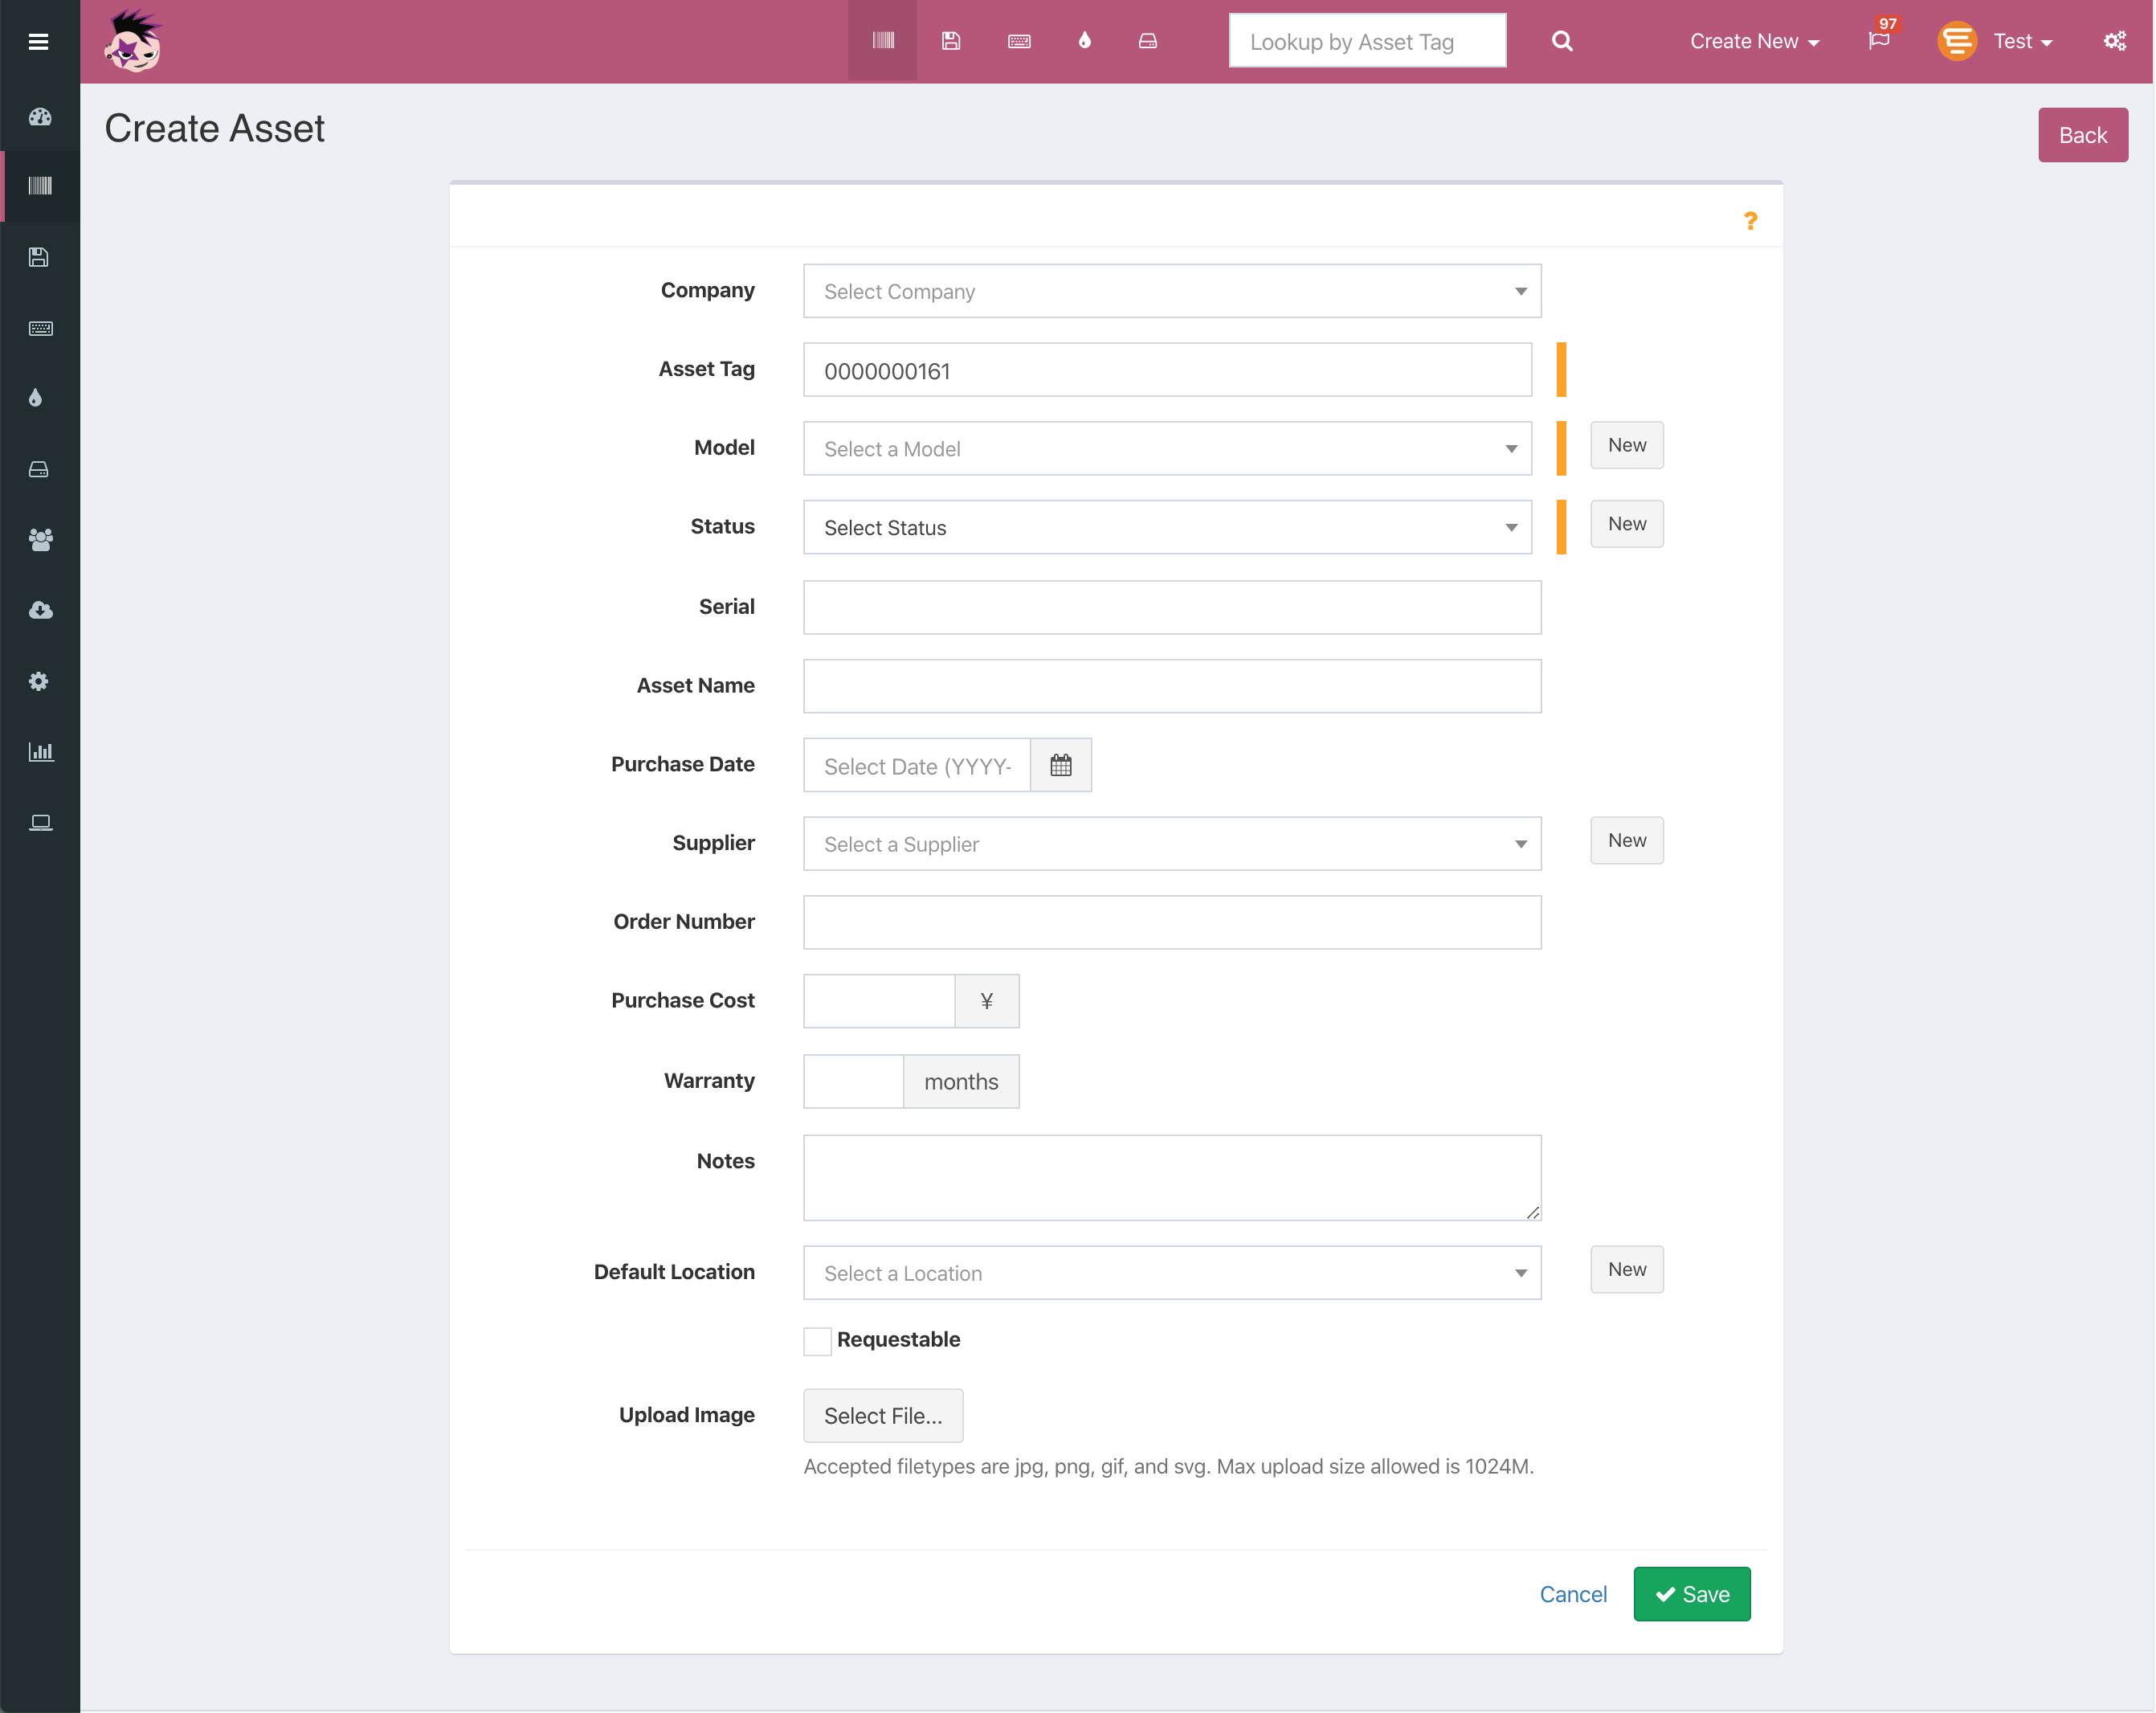
\includegraphics[width=0.9\textwidth]{figures/other-systems/snipeitapp-create-asset-ui-screenshot.png}}
    \caption{Example of an asset management system with too many fields that need to be filled out. \cite{SnipeIT}}
    \label{fig:too-many-fields}
\end{figure}

% Måske GUI vs. Command Prompt? Måske en pointe i at TUI er simplere?
Since the client is experienced computer users, it is relevant to consider what kind of user interface the system should be implemented. A simple option is to use a text-based user interface (TUI), as the employees at the IT department is expected to know how to use a terminal to access the system. The client, however, also wanted all other employees at the zoo to be able to access the system, in order to view the assets, and it is possible that the other departments also will be using the system. Since it cannot be expected that employees at other departments are equally qualified to use a TUI, a graphic user interface (GUI) has been chosen. 
\par
Below are two images of a graphical user interfaces that comply with the clients wishes (see \autoref{fig:add_asset_no_tags} and \autoref{fig:add_asset_with_tags}). These images will form a basis for the final user interface design.
\par
The images show the process of how an asset is added to the system, and how fields are attached to the asset through tags.

\begin{figure}[H]
    \centering
    \frame{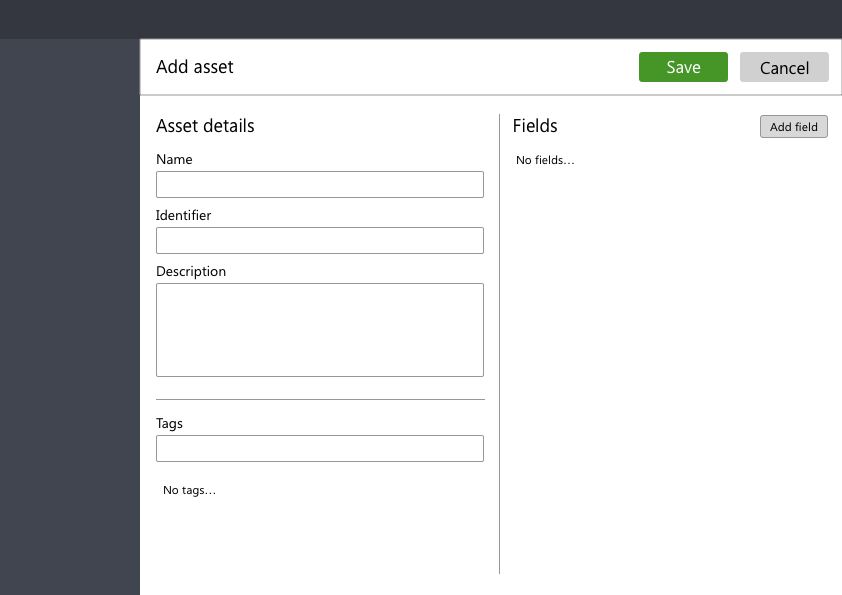
\includegraphics[width=0.9\textwidth]{figures/wireframes/add-asset-no-tags.png}}
    \caption{The process of creating a new asset, at this point no tags or custom fields were added, resulting in no fields beside base fields.}
    \label{fig:add_asset_no_tags}
\end{figure}

\begin{figure}[H]
    \centering
    \frame{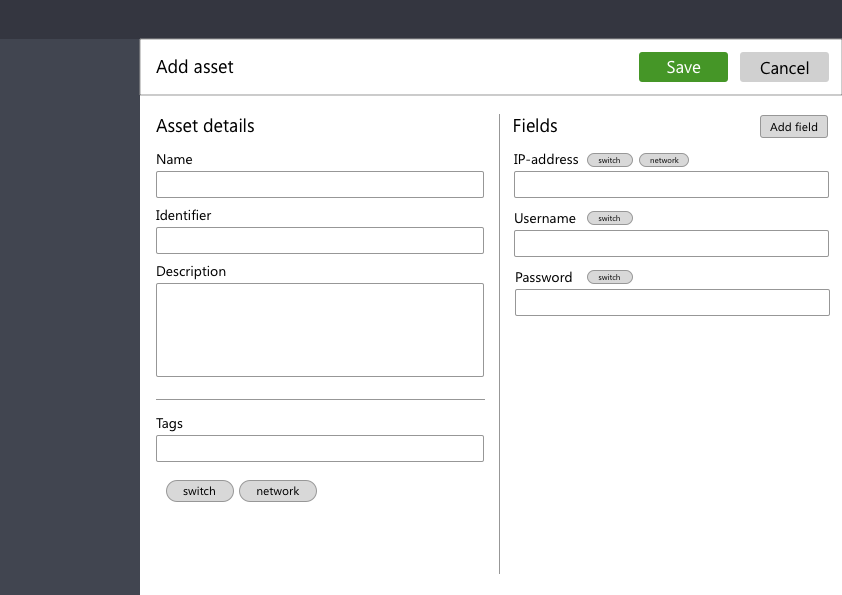
\includegraphics[width=0.9\textwidth]{figures/wireframes/add-asset-with-tags.png}}
    \caption{An example of how the user interface for adding a new asset looks after adding some tags and custom fields.}
    \label{fig:add_asset_with_tags}
\end{figure}

There are two types of users of the system, the administrators (the admin class) of the system and the other employees (the employee class), who have much more restricted access to the system. The images above (\autoref{fig:add_asset_no_tags} and \autoref{fig:add_asset_with_tags}) show the user interface for the admin. If an employee user accesses the system, the interface will be limited with fewer functionalities, as these users are not allowed to make changes to the systems content.

% Summary
\section{Summary} \label{ssc:ad_summary}
In this chapter, the application domain has been analysed. The different actors that will interact with the system have been identified and a number of use cases have been described in order to better understand the purpose of the system. Based on this, essential system functions have been described, which were used to examine the requirements for the user interface the system. 
\par
The analysis has been used in designing the system architecture in the following chapter.


%%%%%%%%%%%%%%%%%%%%%%%%%%%%%%%%%%%%%%%%%%%%%%%%%%%%%%%%%%%%%%%
% Architectural Design
%%%%%%%%%%%%%%%%%%%%%%%%%%%%%%%%%%%%%%%%%%%%%%%%%%%%%%%%%%%%%%%
\chapter{Design} \label{ch:architectural_design}
Through the development of the system, more components and subsystems have been added to the system structure. The system has been split into smaller parts to get a better understanding of its components, and a more detailed class diagram has been constructed. These components and subsystems have been discussed in this chapter.


% Criteria
\section{Criteria} \label{sc:criteria}
In this section the criteria for the system has been prioritized based on the criteria analysis model as described in \cite[chap 9]{OOAD}.

\begin{table}[H]
    \centering
    \resizebox{\textwidth}{!}{%
    \begin{tabular}{|l|c|c|c|c|}
        \hline
        \textbf{Criterion} & \textbf{Very important} & \textbf{Important} & \textbf{Less important} & \textbf{Irrelevant} \\
        \hline
        \hline
        Usable & $\pmb{\times}$ & & & \\
        \hline
        Secure & & & $\pmb{\times}$ & \\
        \hline
        Efficient & & & $\pmb{\times}$ & \\
        \hline
        Correct & $\pmb{\times}$ & & & \\
        \hline
        Reliable & & $\pmb{\times}$ & & \\
        \hline
        Maintainable & & $\pmb{\times}$ & & \\
        \hline
        Testable & & & $\pmb{\times}$ & \\
        \hline
        Flexible & $\pmb{\times}$ & & & \\
        \hline
        Comprehensible & & $\pmb{\times}$ & & \\ 
        \hline
        Reuseable & & & & $\pmb{\times}$ \\
        \hline
        Portable & & & & $\pmb{\times}$ \\
        \hline
        Interoperable & & & & $\pmb{\times}$ \\
        \hline
    \end{tabular}
    }
    \caption{Checklist for prioritizing design criteria}
    \label{tab:my_label}
\end{table}

\textbf{Usable:} One of the primary reasons for Aalborg Zoo to get a system developed from scratch is to get a system that is easy to navigate. Therefore, this is a very important element of the system and the final product. The system is primarily built with usability in focus.

\textbf{Secure:} As the product does not contain any confidential information, security in the system is considered less important. However there is still a minor focus on security, as access to the functions within the program is limited to users with the required permissions and only users within the database can access any thing in the system.

\textbf{Efficient:} The client has expressed that the efficiency of the system is of little concern, so this criteria is considered less relevant. However, it should still be able to complete the tasks within a reasonable amount of time.

\textbf{Correct:} Aalborg Zoo has given weighted requirements for the system, as seen in \autoref{sc:requirements}. It is very important that the requirements are met upon delivering the finished product, so correctness is marked as \textit{Very important}.

\textbf{Reliable:} As part of the heavy focus on the user experience, it is important that the system behaves in a predictable manner, and does this reliably.

\textbf{Maintainable:} The client has expressed a desire for the program to be maintainable, because they want to maintain the system themselves. Because they are not experts in programming, the system should be as easily maintainable as possible, and build on industry standards. They code base should also avoid high reliance on smaller packages, which might lose support in the future.

\textbf{Testable:} As with all other systems, this system should be developed in such a way, that it is testable. This criteria is marked as less important, because it is not the main focus of the project, but it is still regarded as valuable.

\textbf{Flexible:} The client wants to be able to further develop the system after the product is delivered. Therefore it is very important that it is flexible and without too many dependencies. Change of database type is one of the possible future changes to the system.

\textbf{Comprehensible:} The system should be comprehensible, as the less experiences useres should be able to carry out simple tasks in the system easily. High comprehension also allows the client to easily add the functionality they need later on. For this reason, this criterion is important.

\textbf{Reusable:} No part of the system will be used in other systems and therefore, this criterion is irrelevant.

\textbf{Portable:} The system will only be built for a Windows PC, and for this reason, there is no need for the system to be portable. 

\textbf{Interoperable:} The system will not communicate with other systems, beside the database component, which means this criterion is irrelevant for the system.

% Component design
\section{Component Architecture} \label{sc:component_architecture}
With the criteria defined, the overall component architecture of the system can be designed. Below is a diagram of the different components of the system, followed by a description.

\begin{figure}[H]
    \centering
    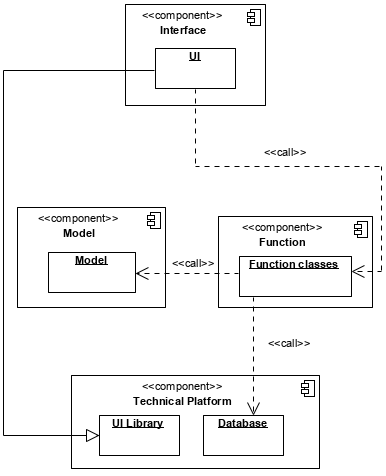
\includegraphics[width=0.6\textwidth]{figures/ComponentDiagrams/ComponentDesignOverview.png}
    \caption{An overview of the overall component design}
    \label{fig:OverviewOfComponentDesign}
\end{figure}
As seen in \autoref{fig:OverviewOfComponentDesign} the architecture of the system closely resembles the "Generic Architecture Pattern" described in \citep[p 198]{OOAD}.
\par
At the bottom is the technical platform, which contains a UI Library and a database. In the center to the left is the model component, which stores the model of the problem domain. To the right of this is the function component, which contains classes, which implements most of the functionality of the system. At the top of the diagram is the interface component, which only contains the UI, as the system will only communicate with the database and the users.
\par
The classes in the model can be utilized and manipulated by the function classes, which is the reason for the call connection between the two subcomponents. These are triggered by interactions between the users and the system in the UI, which is the cause of the call connection between the UI and the function classes. The UI is based off of the UI Library, which means the UI is a specialization of the UI Library. Lastly, the function classes will handle the communication with the database and is therefore connected to it by a call connection.
\par
In the following sections, the different components will be examined and described in further detail.

% Technical Platform
\section{Technical Platform} \label{sc:tech_intro}
This section will go through the two components in the technical platform, and the reasons why these have been chosen over other alternatives. The technical platform of the system consists of a database and a user interface framework. These components have been added to the technical platform of the system to ensure the wanted functionality and a better development phase.
\par
The two components have been implemented through a MySQL database and the Windows Presentation Foundation (WPF) respectively. The reasons for these implementations and how they work have been examined and elaborated upon in this section.
\subsection{Database}\label{ssc:tech_database}
As the system needed to be used on multiple different devices at the same time, a central storage control needed to be implemented. To ensure a reliable storage solution, a database has been chosen to act as the central storage system. Aalborg Zoo currently uses a Microsoft SQL Server 2012, this database server is an older version, which does not support JSON indexation (Allowing JSON elements to be searched as virtual columns \cite{MySQLJSON}). JSON indexation feature allowed for a more versatile system, as well making it possible to implement some of the requirements like "Function tags" \autoref{sc:requirements}, to be implemented at a later date. \\
Because JSON indexation was a requirement for the chosen database, MySQL was chosen as the database for the system. MySQL was chosen because MySQL is a free software, which contains the required functionality for developing the system. As well as its a well know SQL that has a large user base, which results in good first and third party documentation, so its easier for new developers to understand the database. \\

The database is configured as a relational database \cite{RelationalDB} so each element in that database is only present once, and any relation between objects are defined with relations between ID's. This makes the database more storage efficient, but can make it slower than a non relational database, upon scaling. \\

\subsection{Windows Presentation Foundation} \label{ssc:tech_wpf}
The user interface framework used for the system is Windows Presentation Foundation (WPF). Other frameworks were considered, such as Windows Forms (WinForms), which was excluded because the project was focusing on a sophisticated UI where WinForms primarily focus on lightweight UI and giving the developers the ability to quickly get started building applications. 
%https://docs.microsoft.com/en-us/windows/apps/desktop/choose-your-platform
Universal Windows Platform (UWP) was also considered, but was dropped primarily since it only supports Windows 10. WPF also gives the ability to unit test the interface.

%Universal Windows Platform (UWP) was also considered, but as it is used primarily for designing Windows apps and not as much for desktop systems, this was not a viable option \todo{Indsæt kilde på UWP er app orienteret}. \citep{microsoft-choose-your-platform}
%only runs on Windows 10, which Aalborg Zoo might not run on all their systems, this was not a viable option.
\par

Using WPF, the Model-View-ViewModel pattern (MVVM) was the optimal choice for structuring the code \citep{WPFandMVVM}. This pattern is designed to make it easier to swap out the UI while keeping the code behind constant. The pattern is also designed to take advantage of the binding functionality of WPF. \citep{MvvmBasics, Bindings}
\subsection{.NET Core 3} \label{ssc:tech_core}
The system has been written in .NET Core 3. This has been chosen over .NET Framework, because Framework will be phased out in the future, which makes .NET Core 3 more future proof. .NET Core 3 has been developed to replace .NET Framework and with the ambition to make development across different operating systems easier.

% Model component
\section{Model Component} \label{sc:model_component}
Based on the analysis of the problem domain (see \autoref{ch:problemdomain}), through the class diagram, event table, and state charts, the model component of the system has been constructed.
\par
Additional classes, attributes, and structures have been defined to support the mentioned events and the desired functionality of the system. The result is an updated class diagram that contains attributes, operations, and additional classes and structures.

\subsection{Additional classes}
To sufficiently solve the problems in the problem domain, additional classes were needed and have been described.
\par

\subsubsection{\textit{Tag} and \textit{Asset-tag relation}}
During the interviews, Aalborg Zoo mentioned a potential organisational structure to ease the use of the system (see \autoref{ch:problemdomain}). This structure is based on tags, which can be attached to assets and used to filter and add details to these.
The structure adds the \textit{Tag} and \textit{Asset-tag relation} classes to the system. 
\par
A tag will either belong to a department or be available to all departments \autoref{fig:TagAndAsset-TagRelationWithAttributes}.
\par
The \textit{Asset-tag relation} class has been added to represent a connection between an asset and a tag, as an asset can have multiple tags related to it and a tag can be related to multiple assets.
\par

\begin{figure}[H]
    \centering
    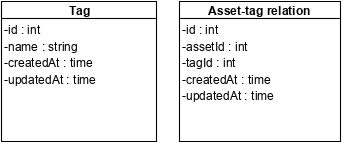
\includegraphics[width=0.55\textwidth]{figures/Classes/TagAndAsset-tagRelationWithAttributes.png}
    \caption{Overview of the \textit{Tag} a \textit{Asset-tag relation} classes with attributes}
    \label{fig:TagAndAsset-TagRelationWithAttributes}
\end{figure}


\subsubsection{\textit{Field}}
To help declutter the application and fulfill the requirement to only fill in relevant information intuitively, the \textit{Field} class is introduced \autoref{fig:FieldWithAttributes}). Both assets and tags can contain the \textit{Field} class. If a field is contained by a tag and that tag is attached to an asset, the field is transferred to the asset as well. Fields only exist in an asset or a tag and never on its own.
\par
The field has certain attributes unique to the class:
\begin{itemize}
    \item \textbf{Type} that defines what kind of input it takes. This can be a text box, a text area, a number, a date, or a checkbox.
    \item \textbf{Content} which will hold the value set by the user.
    \item \textbf{Required} which defines whether or not the field must be filled in before saving the asset
\end{itemize}

\begin{figure}[H]
    \centering
    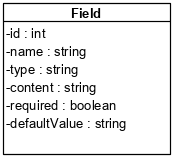
\includegraphics[width=0.28\textwidth]{figures/Classes/FieldAttributes.png}
    \caption{Overview of the \textit{Field} class with attributes}
    \label{fig:FieldWithAttributes}
\end{figure}


\subsubsection{\textit{Comment}}
To allow the users to comment on assets in the system, a \textit{Comment} class has been introduced. A comment is attached to an asset and contains the ID and name of the asset, the username of the user, whom the comment was created by, a comment text, and timestamps for its creation and last update (see \autoref{fig:CommentWithAttributes}).

\begin{figure}[H]
    \centering
    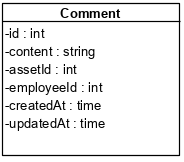
\includegraphics[width=0.28\textwidth]{figures/Classes/CommentAttributes.png}
    \caption{Overview of the \textit{Comment} class with attributes}
    \label{fig:CommentWithAttributes}
\end{figure}


\subsubsection{\textit{FieldContainer}}
To ensure that both the asset and tag classes have a list of fields and has the correct properties and functionality, an abstract class has been implemented called \textit{FieldContainer}. Both the asset and tag classes are specializations of this abstract class (see \autoref{fig:FieldContainer}).

\begin{figure}[H]
    \centering
    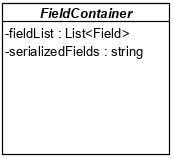
\includegraphics[width=0.28\textwidth]{figures/Classes/FieldContainer.png}
    \caption{Overview of the \textit{FieldContainer} class with attributes}
    \label{fig:FieldContainer}
\end{figure}


\subsubsection{\textit{User}}
To model the users in the system, the class \textit{User} was added. This class contains information about the user, such as username, as well as the users domain (see \autoref{fig:User}).

\begin{figure}[H]
    \centering
    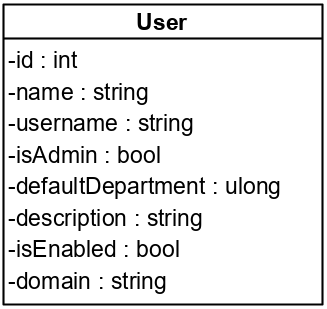
\includegraphics[width=0.28\textwidth]{figures/Classes/User.png}
    \caption{Overview of the \textit{User} class with attributes}
    \label{fig:User}
\end{figure}

Based on these additional classes, the \textit{Employee}, \textit{Admin}, and \textit{Loan} classes needed a revision.
\par
The \textit{Employee} and \textit{Admin} classes have been used to store information about the system's users. This is covered by the \textit{User} class, which also stores information about whether or not that user is an admin.
\par
Aside from this, the \textit{Loan} class has been used to keep track of who is in possession of which assets. This functionality can be covered by the \textit{Tag} class, as it can act as the relation between an asset and a user, by containing the username of the user as its label. This means that an asset can have tags attached, containing the usernames of the employees currently in possession of it.
\par
The other functionality of the \textit{Admin} class has been to identify whether the logged in user has access to administrator functionality or not. This function is handled by the \textit{Session} class, which will be explained in the function component (see \autoref{sc:function_component}).
\par
Based on these changes, the \textit{Admin}, \textit{Employee}, and \textit{Loan} classes from the problem domain have become obsolete and will therefore not be taken into consideration when designing the system.

\subsection{Attributes of problem domain classes}
To ensure that every event and functionality is supported, the following attributes have been added to the classes from the class diagram in the problem domain (see \autoref{fig:FirstPDClassDiagram}).
\par
Throughout this subsection only attributes needing further explanation will be mentioned. Full attribute lists can be found in the related figures of the classes.

\subsubsection{Asset attributes}
An asset has a timestamp of its deletion. This is used for soft deletion, which works as an extra step to avoid unwanted deletes. Soft deletion works by marking an asset with a deletion date, instead of removing the element from the database entirely. This allows the asset to be recovered, if it is accidentally deleted (see \autoref{fig:AssetWithAttributes}).

\begin{figure}[H]
    \centering
    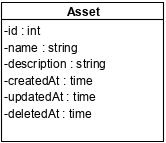
\includegraphics[width=0.28\textwidth]{figures/Classes/AssetAttributes.png}
    \caption{Overview of the \textit{Asset} class with attributes}
    \label{fig:AssetWithAttributes}
\end{figure}

\subsubsection{Department attributes}
The \textit{Department} class does not contain any nontrivial attributes, and can be see in \autoref{fig:DepartmentWithAttributes}.
\begin{figure}[H]
    \centering
    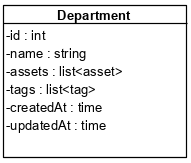
\includegraphics[width=0.28\textwidth]{figures/Classes/DepartmentAttributes.png}
    \caption{Overview of the \textit{Department} class with attributes}
    \label{fig:DepartmentWithAttributes}
\end{figure}


\subsection{Structures}
The events and relations not completely supported by the classes and attributes described previously in this section will be achieved with the following structures of classes.

\subsubsection{Assets and tags can contain fields}
Both the \textit{Asset} and the \textit{Tag} classes aggregates the \textit{Field} class. An asset or a tag can contain multiple fields, but a field belongs to only one asset or one tag. To ensure that both classes have a list of fields and implement the correct properties, they both specialize the abstract class \textit{FieldContainer} (see \autoref{fig:AssetTagFieldStructure}).

\begin{figure}[H]
    \centering
    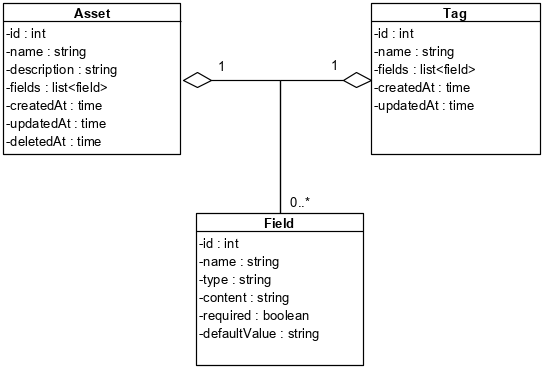
\includegraphics[width=0.65\textwidth]{figures/Structures/AssetTagFieldStructure.png}
    \caption{Overview of the structure between the \textit{Asset}, \textit{Tag}, \textit{FieldContainer}, and \textit{Field} classes}
    \label{fig:AssetTagFieldStructure}
\end{figure}

\newpage

\subsubsection{An asset contains comments}
An asset can be commented on, which attaches the comment to the asset. An asset can have multiple comments, but a comment can only be attached to one asset (see \autoref{fig:AssetCommentStructure}). 
\par
The comments could be implemented as a list on the asset. However, because the comments will be shown in parts of the system without the assets, the aggregation makes it possible to only fetch the comments and sort through these, without having to fetch all the assets as well.

\begin{figure}[H]
    \centering
    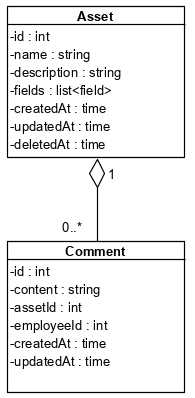
\includegraphics[width=0.25\textwidth]{figures/Structures/AssetCommentStructure.png}
    \caption{Overview of the structure connecting the \textit{Asset} and \textit{Comment} classes}
    \label{fig:AssetCommentStructure}
\end{figure}

% \subsubsection{Tag relation between asset and tag}
% Between the \textit{Tag} and \textit{Asset} classes is a many-to-many relation, which has been replaced by the class \textit{Tagged}. An asset can have multiple tag relations attached to it, as tags can be added to the asset dynamically. A tag does also have multiple tag relations connected to is, as a tag can be attached to multiple assets.

% \begin{figure}[H]
%     \centering
%     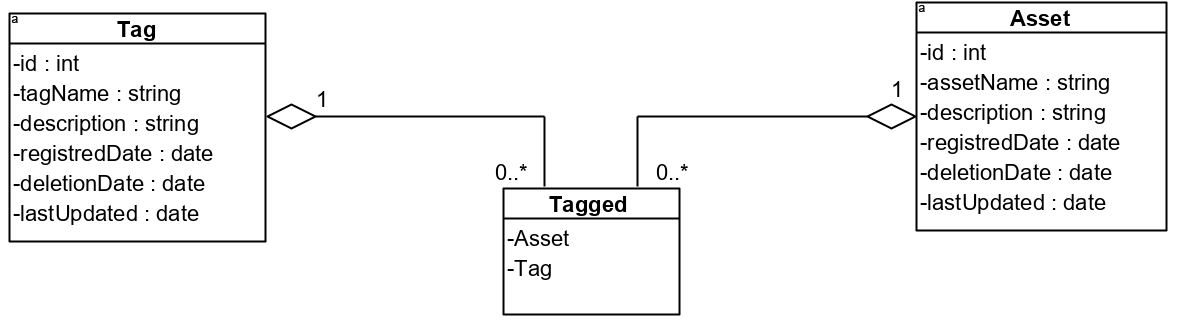
\includegraphics[width=0.8\textwidth]{figures/Structures/TagAssetRelation.PNG}
%     \caption{Overview of the asset class}
%     \label{fig:TagAssetRelation}
% \end{figure}

\subsubsection{A department contains assets and tags}
Assets and tags are added to a department, as they are created. An asset belongs to exactly one department, while a tag belongs to one or all departments. A department contains multiple assets and tags (see \autoref{fig:DepartmentAssetTagStructure}). The tag is depicted to belong to non or 1 department. This should be read as a tag either belongs to one department or belongs to none. When a tag belongs to non, it becomes available to all.

\begin{figure}[H]
    \centering
    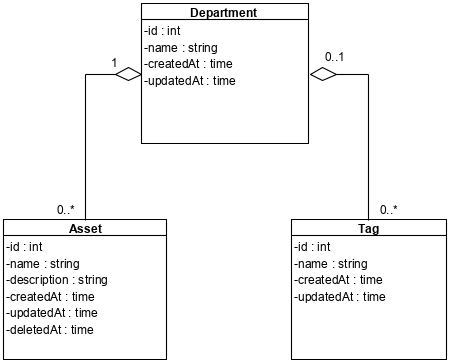
\includegraphics[width=0.7\textwidth]{figures/Structures/DepartmentAssetTagStructure.png}
    \caption{Overview of the structure between the \textit{Department}, \textit{Asset}, and \textit{Tag} classes}
    \label{fig:DepartmentAssetTagStructure}
\end{figure}

\subsubsection{Parent tags}
To make the tagging more manageable, the ability to group tags has been introduced, mimicking a hierarchical folder structure. This is accomplished through parent tags. By doing this, a parent tag can contain multiple tags, which are seen as its children. 
\par
A tag can only either belong to one parent tag or be a parent tag itself. This means that there is no single tag that can act as both parent and child tag. As a product of this, the structure becomes a two level hierarchy (see \autoref{fig:TagHierarchy}). 
\par
The figure (see \autoref{fig:TagHierarchy}) is only an illustration of the relation between two tags. In the system the two classes exist as the \textit{Tag} class, with the relation represented by an attribute linking the child tag to the parent.

\begin{figure}[H]
    \centering
    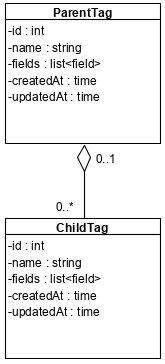
\includegraphics[width=0.28\textwidth]{figures/Structures/TagHierarchy.png}
    \caption{Overview of the structure of the \textit{ParentTag} and \textit{ChildTag} classes}
    \label{fig:TagHierarchy}
\end{figure}

\newpage

\subsection{Updated class-diagram}
The additions mentioned above have added up to the following class-diagram, which represents the model component, and can be seen in \autoref{fig:ModelComponentClassDiagram}.

% Tags og andre ting skal introduceres inden dette afsnit
\begin{figure}[H]
    \centering
    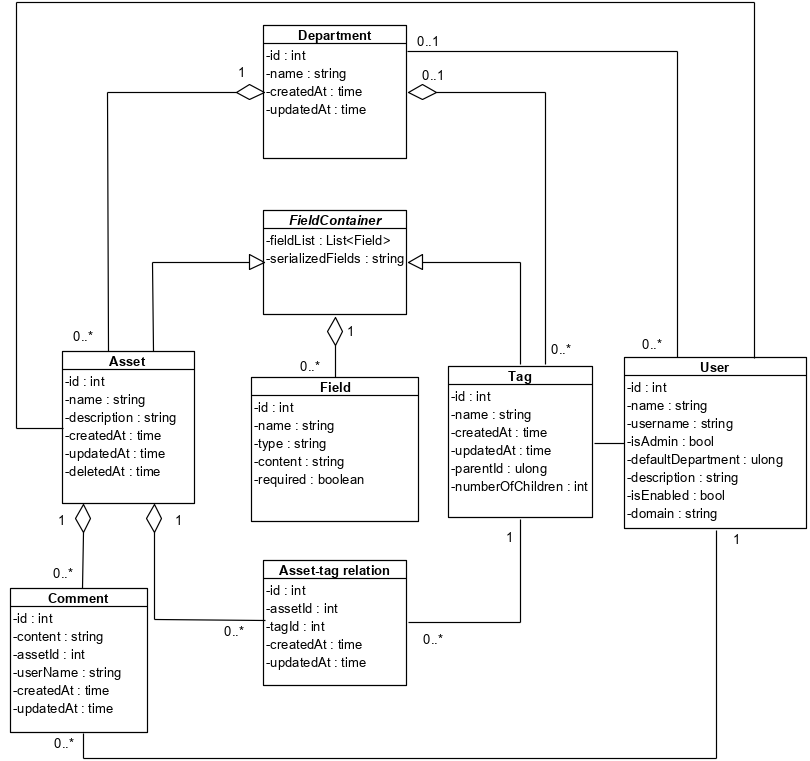
\includegraphics[width=0.9\textwidth]{figures/ClassDiagrams/ModelComponentClassDiagram.png}
    \caption{Class diagram for the model component}
    \label{fig:ModelComponentClassDiagram}
\end{figure}


% Function component
\section{Function Component} \label{sc:function_component}
Having added new attributes, classes, and structures to the class diagram through the model component, the functions from the function list can be implemented as well. Some of these functions should be implemented in the classes directly, others should be placed in the function component. The following section contains additions to the original function list, the arguments for these additions, decisions about implementations of these, and the final function component design.
\par
Throughout this sections, only the most essential functionalities will be described. There are smaller classes that have responsibilities less essential to the core functionality of the system, which will not be described.

\subsection{Additions to the function list}
The function list (see \autoref{tab:functions} on page \pageref{tab:functions}) has been constructed based on the original class diagram (see \autoref{fig:FirstPDClassDiagram}), but does not accommodate the new additions from the model component. To support the new classes, the following functions have been added:

\begin{table}[H]
\centering
    \begin{tabular}{|c|l|l|l|}
        \hline
        \textbf{Nr.} & \textbf{Function name} & \textbf{Complexity} & \textbf{Function type}\\
        \hline
        1 & Get asset by id & Simple & Read\\
        \hline
        2 & Get department by id & Simple & Read\\
        \hline
        3 & Get tag by id & Simple & Read\\
        \hline
        4 & Search for tag & Medium & Compute/Read\\
        \hline
        5 & Add field to asset/tag & Medium & Update\\
        \hline
        6 & Update tag information & Simple & Update\\
        \hline
        7 & Update department information & Simple & Update\\
        \hline
        8 & Tag created & Simple & Update\\
        \hline
        9 & Tag deleted & Simple & Update\\
        \hline
        10 & Tag attached & Medium & Update\\
        \hline
        11 & Tag detached & Medium & Update\\
        \hline
    \end{tabular}
\end{table}

Functions 1-3 are added to read the objects from the model to the application domain. The \textit{Get asset by id} function replaces the \textit{View asset} function, as they both fetch the object.
\par
Function 4 makes it possible to search for a tag, in the same way as it is possible to search for an asset.
\par
Function 5 makes it possible to add a field to an asset or a tag.
\par
Functions 6 and 7 handle the updating of the tags and departments in the system. This lets the user maintain the tags and departments, as they change name or, for the tags, need more functionality.

\subsection{Design}
The following includes examinations of the functions and design decisions about how they should be incorporated in the component design. To better separate the responsibility of the different classes, the \textit{Asset}, \textit{Comment}, \textit{Department}, \textit{Field}, \textit{User}, and \textit{Tag} classes have been implemented as simple data classes. This means that they will simply store data and only perform operations related to interpreting the data of the model.

\subsubsection{Maintaining the model}
All the \textit{add}, \textit{remove}, \textit{update}, and \textit{get by id} functions are used by an employee with admin status. These functions should be handled similarly for assets, departments, users, and tags, and therefore they will all be grouped into a strategy \citep{OOAD}. A thorough look at these functions and the structure will show that this pattern is actually a repository pattern \citep{RepositoryPatternDescription}.
\par
An intuitive name of the class describing the overall strategy is \textit{Repository}. The class is abstract, as every class acting as a concrete strategy will inherit the functions from the \textit{Repository}. The concrete classes handle the assets, departments, users and tags respectively and have been named: \textit{AssetRepository}, \textit{DepartmentRepository}, \textit{UserRepository}, and \textit{TagRepository}. These control the maintenance of the data for their designated classes in the model.
\par
As mentioned, these concrete classes have operations for adding, removing, and updating, which all take an object of the designated class, and an operation for getting an object by id. This structure has been placed in the function component, as it does not belong to a specific class in the model component. 
\begin{figure}[H]
    \centering
    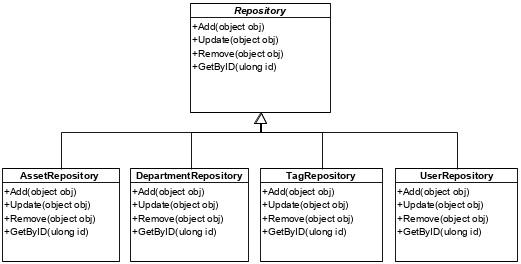
\includegraphics[width=0.85\textwidth]{figures/FunctionComponent/Repository_pattern.png}
    \caption{The repository pattern for maintaining data in the model}
    \label{fig:RepositoryPattern}
\end{figure}

\subsubsection{Attach and detach tag}
The operations of attaching or detaching a tag to or from an asset is called by an admin and involves the \textit{Tag} and \textit{Asset} classes. The functions create or delete an instance of the \textit{Asset-tag relation} class containing the involved asset and tag. The operations should be added to a class in the function component, as the admin does not carry out the operations.
\par
The operations have been placed in the \textit{AssetRepository} class, as the asset is responsible for maintaining the connections to its attached tags. Placing them directly on the \textit{Asset} class, however, would give the class responsibility of an operation in which it participates solely as an object. The operations have been named \textit{AttachTags} and \textit{DetachTags}. Both operations take two parameters, an asset, and a list of tags to be attached to the asset.

\begin{figure}[H]
    \centering
    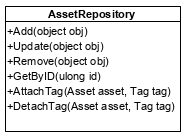
\includegraphics[width=0.3\textwidth]{figures/FunctionComponent/AttachTag.png}
    \caption{The \textit{AssetRepository} class with the \textit{AttachTag} and \textit{DetachTag} operations}
    \label{fig:AttachDetachTag}
\end{figure}

\subsubsection{Search for asset or tag}
The \textit{search for asset} function lets the user search through the assets in the system and returns the assets that comply with the search query. Multiple assets are handled and therefore it would not be intuitive to add it as an operation on the asset class. It is called by the user, but the user is not responsible for searching through the assets, so the function has been placed as an operation in the function component.
\par
The function \textit{search for tag} goes through the same process and both functions have the same structure. The search is carried out on the elements in the database and therefore they fit well into the specialized classes of the \textit{Repository} class.

\begin{figure}[H]
    \centering
    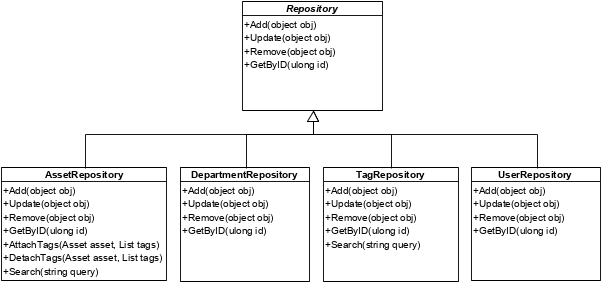
\includegraphics[width=0.92\textwidth]{figures/FunctionComponent/Repository_pattern_with_search.png}
    \caption{The repository pattern with the search operations for assets and tags}
    \label{fig:RepositoryPatternWithSearch}
\end{figure}

\subsubsection{Comment asset}
Commenting on an asset adds a comment to the asset. It is desired that the comments can be retrieved and shown without retrieving the entire asset, to which it belongs. The reason for this is that the newest comments are to be shown on the home page of all admins, to give an overview of the latest changes and problems. Therefore the comments will not be placed directly on the asset, but will be stored separately and contain a relation to the asset. Because of this, the comment will need the functions \textit{add}, \textit{remove}, \textit{update}, and \textit{get by id} and can therefore be seen as another specialized class of the \textit{Repository} class.

\begin{figure}[H]
    \centering
    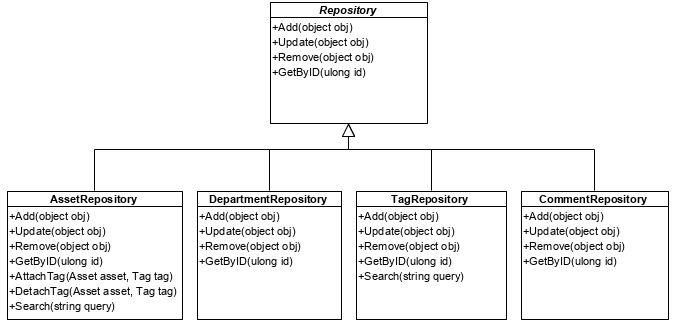
\includegraphics[width=1\textwidth]{figures/FunctionComponent/CommentRepository.png}
    \caption{The repository pattern with the \textit{CommentRepository}}
    \label{fig:RepositoryPatternWithCommentRepository}
\end{figure}

\subsubsection{Authenticate user \& Check access level}
As mentioned in \autoref{sc:model_component}, the \textit{Employee} and \textit{Admin} classes are used to differentiate between users with and without administrative access to the system. This should not be handled by the models themselves, which has let to the creation of a new class in the function component called \textit{Session}. This, in combination with the addition of the \textit{Tag} class, makes the \textit{Admin} and \textit{Employee} classes obsolete.
\par
The operations for authenticating and checking access level of users have been named \textit{Authenticated} and \textit{IsAdmin}. \\
The \textit{Session} class also contains the attributes \textit{Username} and \textit{Domain}, to make sure that the information about the employee currently logged in is available to the system.

\begin{figure}[H]
    \centering
    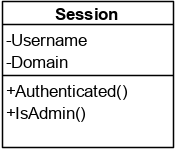
\includegraphics[width=0.22\textwidth]{figures/FunctionComponent/Session.png}
    \caption{The \textit{Session} class}
    \label{fig:session_class}
\end{figure}

% \subsubsection{Export report}
% The operation has been placed in a class in the function component named \textit{ExportHandler}.
% \begin{figure}[H]
%     \centering
%     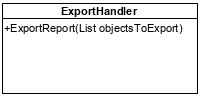
\includegraphics[width=0.4\textwidth]{figures/FunctionComponent/ExportHandler.png}
%     \caption{The \textit{ExportHandler} class}
%     \label{fig:ExportHandler}
% \end{figure}

\subsubsection{Updating data classes}
To ensure that the data in the data classes is handled correctly, controllers have been introduced between the data classes and the related classes in the function component. This ensures that the data is correctly handled and valid, before saving it to the data classes.
\par
The controllers handle communication with classes that either need information from the data classes or change some of the information. They also handle communication with the repositories. This makes it possible to call methods in a controller, which then formats the data class and sends them to the associated repository.
\par
The controllers differ in functionality and therefore does not build on a generalized controller. Two controllers have been depicted in the picture below (see \autoref{fig:AssetControllerAndAssetListControllerClasses}).

\begin{figure}[H]
    \centering
    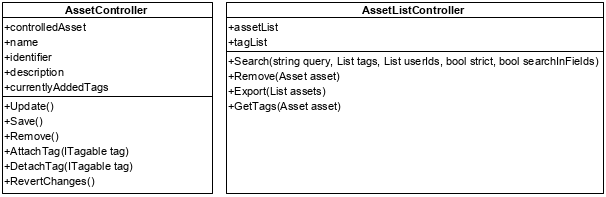
\includegraphics[width=0.95\textwidth]{figures/FunctionComponent/AssetControllerAndAssetListController.png}
    \caption{The \textit{AssetController} and \textit{AssetListController} classes}
    \label{fig:AssetControllerAndAssetListControllerClasses}
\end{figure}

The \textit{AssetController} handles only one asset and gives the dependent classes access to the operation they need, in context of reading and updating the asset. One of these is the \textit{Save} operation, which simply calls the \textit{AssetRepository} with the controlled asset. This way, the surrounding classes do not need any knowledge of the repository doing the operation  save the asset.
\par
The \textit{AssetListController} contains a list of assets and makes it possible for the dependent classes to interact with the list, such as searching through the list and removing an asset from the list. As mentioned above, the controller makes it possible for the dependent classes to ignore the existence of certain classes, such as the repositories.

\subsubsection{Add or remove field to asset or tag}
Adding a field to either an asset or a tag will create a field directly on the asset or tag. The fields do not have their separate place in the system, as they are not relevant without either the asset or the tag, to which they belong. Therefore the function has been implemented in the function component as an operation in an abstract class called \textit{FieldListController}.
\par
The class defines operations such as adding or removing a field to or from a data class (see \autoref{fig:FieldListController}).

\begin{figure}[H]
    \centering
    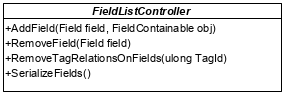
\includegraphics[width=0.5\textwidth]{figures/FunctionComponent/FieldListController.png}
    \caption{The \textit{FieldListController} class}
    \label{fig:FieldListController}
\end{figure}

\subsubsection{Additional classes}
Other classes have been added but are not included in the previous description, as they are not part of the core functionality. The functionality of these classes include logging changes, which is handled by the \textit{Logger} class and saved using the \textit{LogRepository} class. Others are the \textit{Exporter} class handling exporting items from the system, the \textit{FileEncryption} class that secures the application database credentials, and the \textit{UserImporter} that imports users to the system, from a CSV file. The mentioned classes are not implementing core functionality and are therefore not shown in the component diagram either (see \autoref{fig:FunctionComponent}).

\subsection{Function component diagram}
Based on the decisions made in this section, the function component has been constructed and is illustrated in \autoref{fig:FunctionComponent}.

\begin{figure}[H]
    \centering
    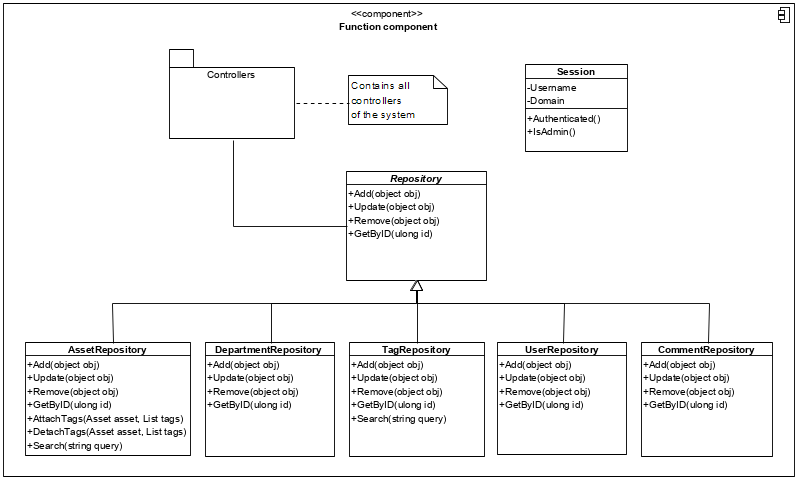
\includegraphics[width=\textwidth]{figures/FunctionComponent/FunctionComponent.png}
    \caption{Illustration of the function component of the system}
    \label{fig:FunctionComponent}
\end{figure}

The overall behaviour of the system is pretty simple, as it only has the state \textit{active}. Therefore, a diagram of this behaviour is trivial and has not been included here.
\newpage

%Connecting component
\section{Connecting Components} \label{sc:connecting_components}
The components have been defined in the above sections and their connections and desired interactions will be described and depicted in the following section.
\par
The model and function components have a few dependencies between them. These dependencies have been converted to connections in a way that gives the most cohesion in the system and the lowest coupling. On top of these criteria, an intuitive design and connection between the components have been striven towards.
\par
The connection between the \textit{Asset}, \textit{Tag}, and \textit{Department} classes and the \textit{Repository} strategy is an aggregation. This is because the concrete strategies handle objects of their designated type as a collection and will contain multiple instances of the class.
\par
The user interface component has a connection to the \textit{Session} class in the function component to ensure that the user can only access the functions belonging to the session. The connection exists as a call, because the relation's only purpose is to ensure that the user's information is available to the system.
\par
The user interface component is also connected with a call relation to the \textit{ExportHandler} class, as the user, if they have admin access, simply calls the function within the \textit{ExportHandler} to export a list of assets.
\par
The \textit{FieldController} contains the functionality to add fields to objects that allow it. The user, if they have admin access, should have access to this functionality and therefore, the user interface has a call relation to the \textit{FieldController} in the function component.
\par
The repository strategy has a connection to the database, to save the different models in the database. This is simply a call relation, as the repositories just need to call the operations on the database.
\\\\
The above descriptions has described the connections between the model and function components. The decisions reasoned above have resulted in the following component diagram.

\begin{figure}[H]
    \centering
    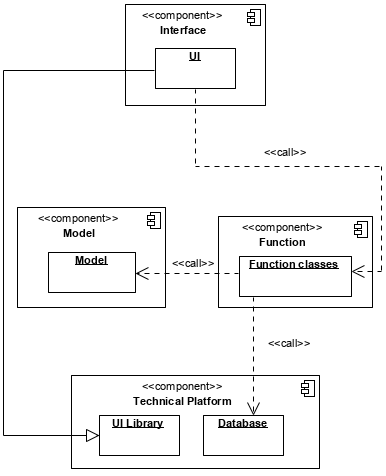
\includegraphics[width=0.8\textwidth]{figures/ComponentDiagrams/ComponentDesignOverview.png}
    \caption{Illustration of the component design of the system}
    \label{fig:FinalComponentDesign}
\end{figure}

\todo[inline]{Actual connection of components diagram}

With the component design constructed and illustrated, the UI can be designed. The UI design will build on the component design and the results from the previous analysis.

%%%%%%%%%%%%%%%%%%%%%%%%%%%%%%%%%%%%%%%%%%%%%%%%%%%%%%%%%%%%%%%
% UI Design
%%%%%%%%%%%%%%%%%%%%%%%%%%%%%%%%%%%%%%%%%%%%%%%%%%%%%%%%%%%%%%%
\chapter{UI Design} \label{ch:ui_design}\todo[inline]{Figurer skal opdateres}
The UI has been designed based on the model and function components, and with the client's wishes to have a functional and simplistic design, in mind. This approach is more functionality oriented, than making the UI and then basing the model and function components on that. The design has drawn inspiration from GitHub's \citep{GithubDesktop} desktop application and Overleaf's online LaTeX editor \citep{Overleaf}, as their designs are very simple and their color pallets are made up of low saturation colors. 
\par

The user interface has been designed based on a modern minimalistic design \citep{MinimalistUX} as this was a requirement from the client (see \autoref{sc:requirements}). This means that the design is flat and without a lot of shadows. Many of the corners in the application have been rounded for a milder look and the colors are very similar.

\section{Client feedback}
As mentioned above, the ideal UI, as described by the client, is simple and effective. This criteria has led to a UI with a limited set of colors, a cohesive design across the interface, and functionalities based on standards within the clients work environment, in this case Microsoft Windows. This is, for example, reflected in the way selecting elements in a list is similar to how it is done in Windows.
\par
Some things have been changed a bit from how they are handled in Windows, such as the before mentioned selection of elements in a list. On top of the standard Windows multi-selection, checkboxes have been implemented to make multi-select possible without holding down the 'Ctrl' key. The client can still use the basic Windows method, but will be able to take advantage of the checkboxes as well.

\subsection{Wireframes}
To ensure the compatibility between the clients workflow and the design, wireframes have been developed. Wireframes are an alternative to sketching designs on paper and then turning physical pages, as the user interacts with the system. The wireframes have been shown to the client in the early stages of the project to get feedback and improve the design, before starting to coding functional prototypes.
\par
The wireframes have given a common basis for the further development of the system as well as the UI. One of the things that were illustrated in the wireframes was the page with the list of all assets in the system. This is one of the main pages of the system, as it will be used to access a specific asset, as well as search through, delete, edit, and print out a list of the assets. The wireframe is very simple and only uses black, white, and gray (see \autoref{fig:AssetList_Wireframe}).

\begin{figure}[H]
    \centering
    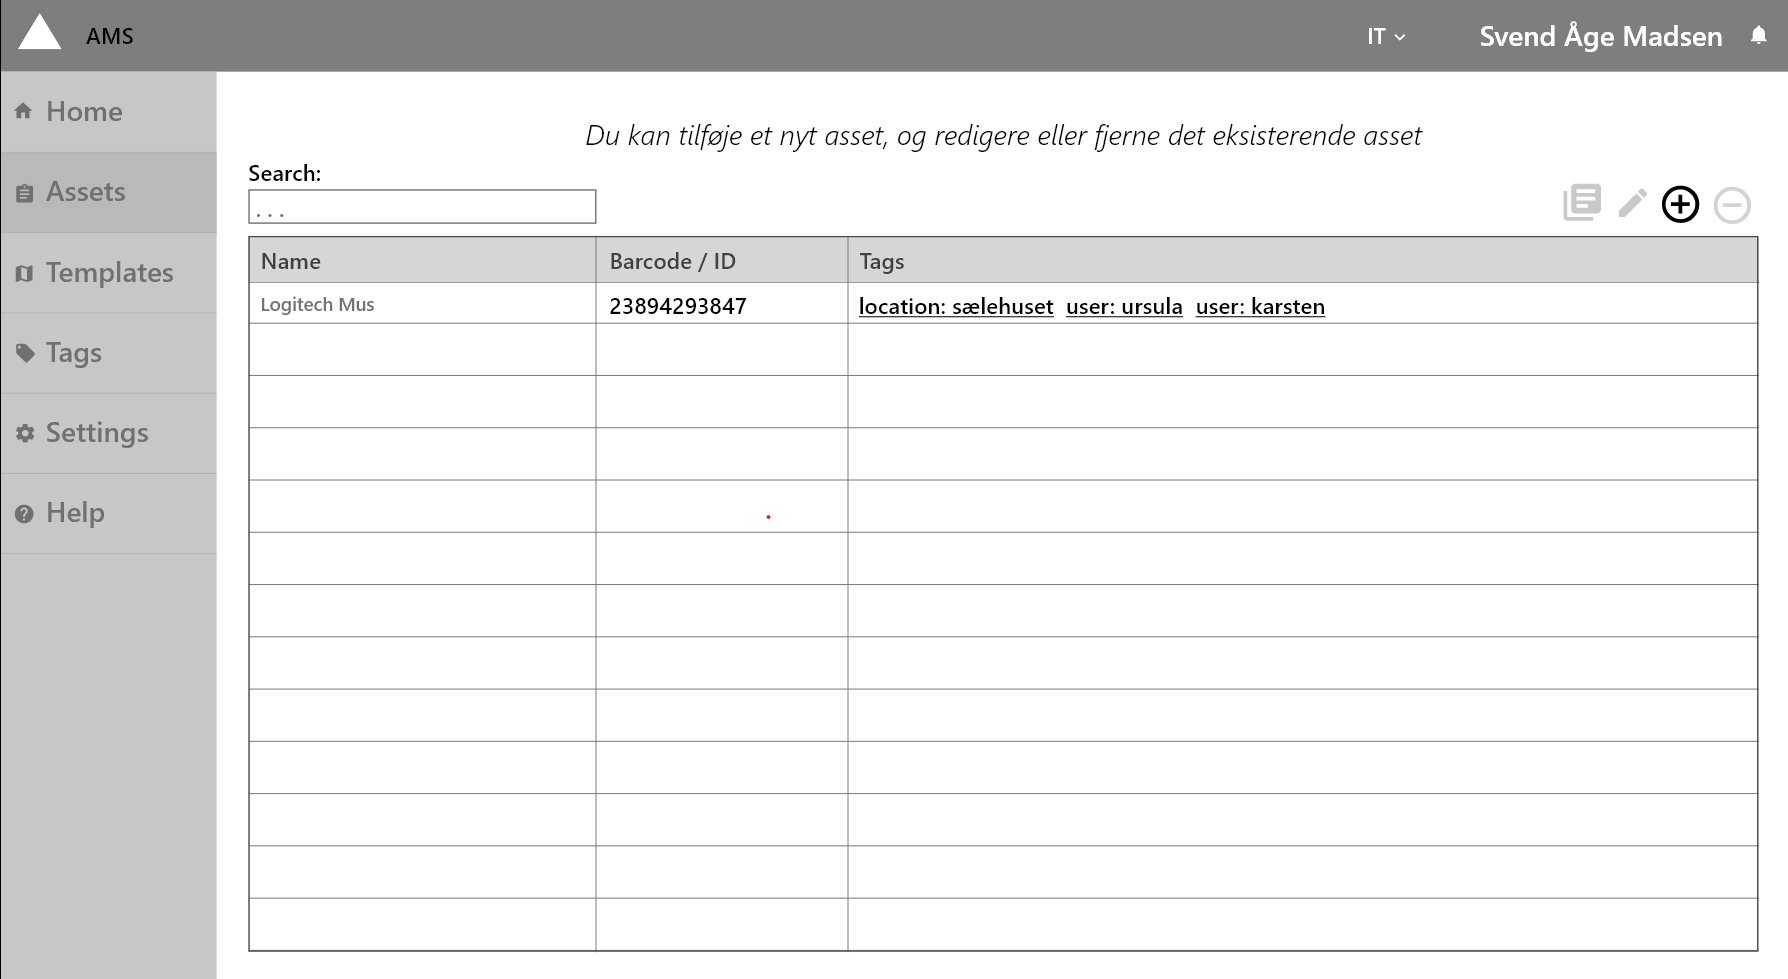
\includegraphics[width=0.8\textwidth]{figures/wireframes/AssetList_Wireframe.png}
    \caption{Wireframe of the AssetList page}
    \label{fig:AssetList_Wireframe}
\end{figure}

Another one of the essential pages is the one used for creating and editing an asset. This page has been illustrated with a few more elements than the list page, as it was important to show the client how it would look after an asset had been assigned several tags and fields. This was important, as the clutter a lot of fields could result in, has been the reason for the client to get a custom system, instead of going with an already existing solution \todo[inline]{Reference to the place where we define the clutter as a problem}. 
\par
The dark grey header and side navigation are consistent across all pages, as they contain functionality that should be available to the user at all times. The asset editor page also contains a number of fields and attached tags, as this is another specific request from the client (see \autoref{fig:AssetEditor_Wireframe}).

\begin{figure}[H]
    \centering
    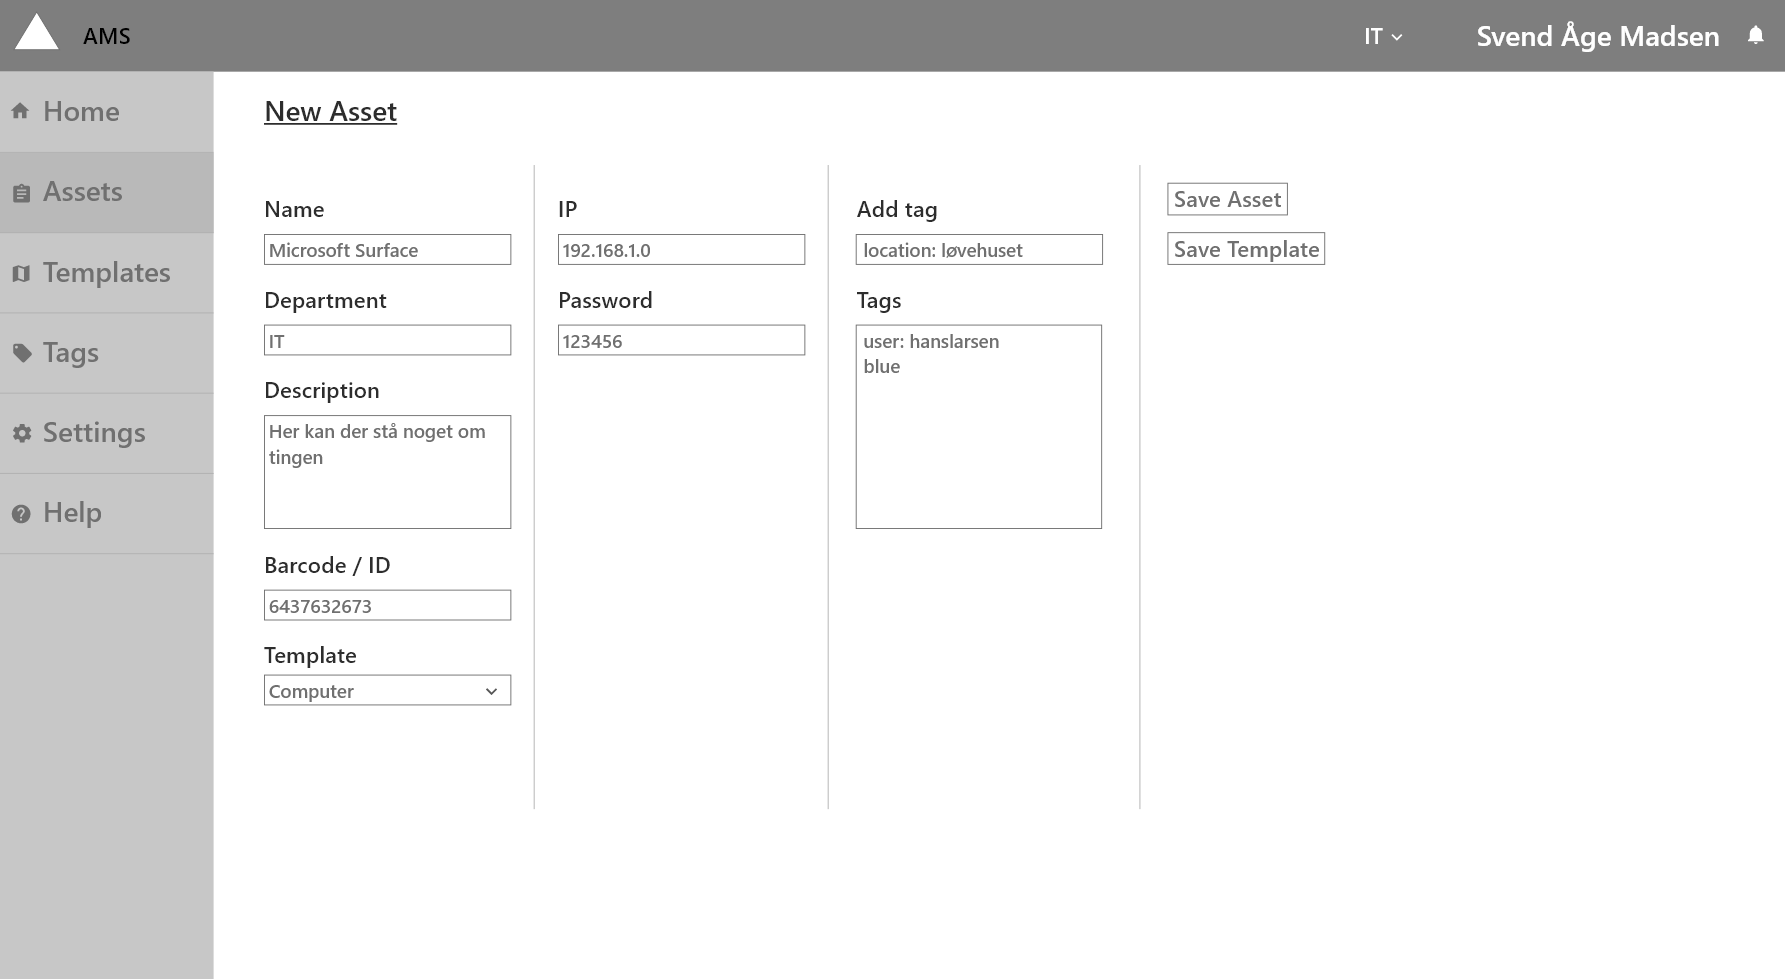
\includegraphics[width=0.8\textwidth]{figures/wireframes/AssetEditor_Wireframe.png}
    \caption{Wireframe of the AssetEditor page}
    \label{fig:AssetEditor_Wireframe}
\end{figure}

The wireframes were well received by the client, as they were very simple and had low saturation. The relatively few elements on the pages also followed the requirements from the client (see \autoref{sc:requirements}).

\subsection{Prototypes}
Based on the wireframes, multiple prototypes have been constructed to show the functionality in action. These prototypes include a visualization of the tagging of assets, which was written in Javascript (see \autoref{fig:PrototypeOfTagging}), as well as a limited, simple version of the system written in HTML, CSS, and Javascript (see \autoref{fig:PrototypeOfSystem}). This method of creating simple prototypes made it possible to show the client the system in a browser, as prototyping in HTML and Javascript is a faster way of creating a visual prototype.
\par
The problem with this method was that the code had to be written in both C\# and Javascript, and two different programming languages might have different limitations. The implementation of certain functions might therefore be more difficult in one language compared to another.
\par
The tagging prototype (see \autoref{fig:PrototypeOfTagging}) was important, as the experience of tagging has been hard to depict. This is primarily because a similar tagging system haven't been found in another system, and therefore had to be made from scratch. Because of this the main purpose of this prototype has been to understand how the client intended to use the functionality in the final product. Especially the keyboard shortcuts that the client tried to use to accomplish different actions, were noted for later implementation in the system. Actions such as entering a parent tag to attach the child tags, stepping out of the parent tag when pressing backspace without anything in the field, and how to show attached tags beneath the field.

\begin{figure}[H]
    \centering
    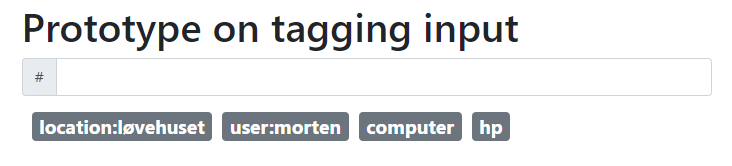
\includegraphics[width=0.8\textwidth]{figures/Prototypes/PrototypeOfTagging.png}
    \caption{Prototype of tagging}
    \label{fig:PrototypeOfTagging}
\end{figure}

The client had a few ideas related to the actions of different keyboard shortcuts, which were implemented in the final system. These include the list of suggestions beneath the field, which automatically updates itself every time a key is pressed, as well as pressing the tab key to auto fill with the first element in the shown list.
\par
To accompany the prototype of the tagging, the client has been shown a prototype of the overall design of the system as well. This prototype was, as mentioned above, written in HTML, CSS, and Javascript and implemented some overall functions such as adding an asset, viewing the information of an asset, and adding fields to the asset. The prototype was not connected to a database and the actions were only for illustrative purposes with no actual effects. \autoref{fig:PrototypeOfSystem} depicts the page for editing an asset in the prototype.

\begin{figure}[H]
    \centering
    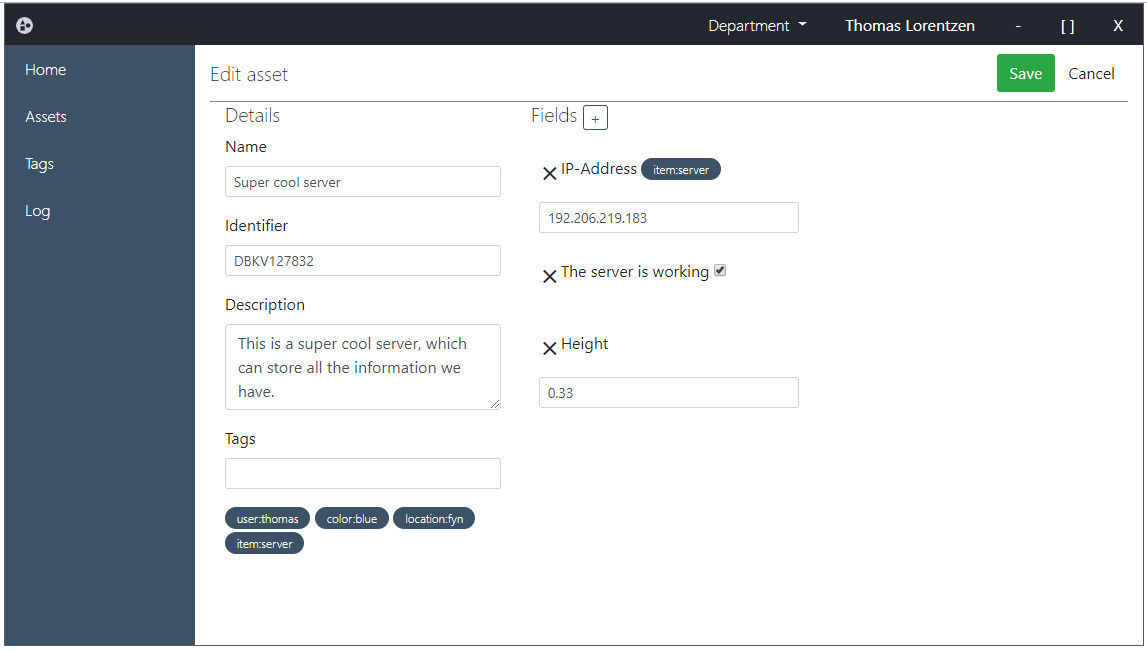
\includegraphics[width=0.8\textwidth]{figures/Prototypes/AssetEditor_Prototype.png}
    \caption{Prototype of system}
    \label{fig:PrototypeOfSystem}
\end{figure}

The client was very pleased with the designs of the prototypes and therefore they have been used as a basis for the final design.

\subsection{Early usability tests}
Based on the feedback from the wireframes and prototypes, the parts depicted in the wireframes and prototypes were developed. A usability test of the early version of the system was done with the client, before too many details and functionalities were implemented. This was done to ensure that the client agreed with the direction in which the functionality and design of the system was headed. 
\par
Another usability test was also performed on a participant with no previous knowledge of the system, but with experience within IT, in order to evaluate the usability of the design as a whole. This was done before the test with the client, which also provided some experience with doing usability tests before involving the client. A screenshot of the system during the usability tests can be seen below (see \autoref{fig:UsabilityTestsEditAssetPage}).

\begin{figure}[H]
    \centering
    \includegraphics[width=0.8\textwidth]{figures/PicturesOfTheSystem/Usabilitytest_editAsset.png}
    \caption{A screen shot of the 'edit asset' page from the usability test}
    \label{fig:UsabilityTestsEditAssetPage}
\end{figure}

One of the things that became clear through the usability tests in the early stages of the system development, was that our participants' intuition, when asked to remove an asset from the system, was to navigate to the edit page of the specific asset and then delete it from there. As seen in \autoref{fig:UsabilityTestsEditAssetPage}, there is no button on the edit page that supports this functionality.
\par
The system only supported removal of an asset from the list page (see \autoref{fig:UsabilityTestsAssetListPage}), but this was not as intuitive to the test participants. Therefore a 'Remove' button was added to the 'Edit asset' page in the final design (see \todo{Insert reference to finished system design of edit asset page}).

\begin{figure}[H]
    \centering
    \includegraphics[width=0.8\textwidth]{figures/PicturesOfTheSystem/Usabilitytest_AssetList.png}
    \caption{A screenshot of the 'asset list' page from the usability test. The 'Remove' button is red, when the mouse is hovering over it, and is just black text when the mouse is not hovering over it.}
    \label{fig:UsabilityTestsAssetListPage}
\end{figure}

Multiple other functionalities and alterations to the design have been implemented in the final product based on the usability tests and the above example is only one of them.
\par
The client was again very pleased with the design of the interface, even though multiple functions had yet to be added and updated to better accommodate usability and the workflow of the client.

\section{Final design}
The final design of the user interface has been developed based on the feedback from the client and other usability test participants as well as the early sketches and prototypes.

\subsection{Overall concepts}
The UI has been designed with cohesion in mind to give the impression of a connected system. Some of the ways this has been achieved are through the color pallet, the simplicity across all the different pages, the left and top menu bars, the positions of buttons, and consistent fonts and font sizes.
\par
The UI has also been developed to be as intuitive to the client as possible. Achieving this has been difficult, but as the client is a Windows user with experience in different enterprise applications, the system implements as many shortcuts and functions native to the Windows platform as possible, in order to support the client's natural workflow.
\par
The design has also been developed in such a way that it accommodates the user's memory and attention span. This is apparent in the way the user never needs to remember the previous steps when using the system. There are no pages, where the information from the previous page is crucial, and the tags make it possible to group similar assets, to make them easier to find through the search function on the list page. As well as making it easier to create similar assets.
\par
The interface accommodates the attention span of the user by making it possible to save progress and return to the task later, in most of the scenarios. This is important, as the user might be distracted during their interactions with the system.
\par
Some of the areas of the design have been described in further detail below.

\subsubsection*{Navigation}
Navigating the system is very important, as the system supports a few different elements, which are handled on different pages. To make the navigation faster and more intuitive to the client, the left menu bar is visible from anywhere within the application. Through this, the pages for the different elements are accessible. The navigation bar also ensures that each page is at most three clicks away from anywhere within the application (see \autoref{fig:UIStructure}).
\par
For example if the user wants to see a specific asset, they press the 'Assets' tab in the navigation menu which will take them to the 'Asset list' page. From here they can remove assets, or access the 'View' or 'Edit' pages for every asset. If the asset is too far down the list or difficult to find, the user can use the search bar to find the asset.

\begin{figure}[H]
    \centering
    \includegraphics[width=1\textwidth]{figures/UIDesignElements/UI_Design_Structure.png}
    \caption{Diagram of the navigation structure of the system}
    \label{fig:UIStructure}
\end{figure}
\todo{Shortcuts?}

Besides this, navigating to the subpages, such as the 'View asset' page, is possible in multiple ways. When the user wants to view an asset, they can double click the asset in the list, press the eye symbol in the right side of the list element, or select it and then press either 'Enter' or 'Ctrl' + 'W'. This gives the user the ability to navigate the interface in the way that is intuitive to them.
\par
Because of the limited number of steps between the different pages, the only type of breadcrumb implemented is the highlighting of the page on the side bar that the user is currently on. If the page layout had multiple steps, a location-based page hierarchy could be shown in the top of the window \citep{Breadcrumbs}.

\subsection{Design methods}
In the design of the UI, a few different design methods and theories have been used. The usage of some of these have been described below.

\subsubsection*{Color}
The color pallet was heavily inspired by the GitHub desktop application and the Overleaf LaTeX editor \citep{GithubDesktop} \citep{Overleaf}. The inspirations have been drawn in order to save time on color selections for every part of the system, and these specific examples have been chosen due to their low saturation and very mild color pallet.

\begin{figure}[H]
    \centering
    \includegraphics[width=0.8\textwidth]{figures/UIDesignElements/GitHub_Desktop_Screenshot.png}
    \caption{Screenshot of the GitHub desktop application \citep{GithubDesktop}}
    \label{fig:GitHubDesktop}
\end{figure}

For the buttons of the application, the dark border and white center was chosen for buttons that did not need to draw a lot of attention. The border is to illustrate the boundaries of the buttons.
\par
When the user hovers over any of the buttons in the application, the color changes to the color of the top menu bar, except the "remove" buttons, as these needs to stand out. This gives the user clarity about whether or not the button is clickable and that the cursor is pointing at it (see \autoref{fig:HoverColorAndBorderedButtons}).

\begin{figure}[H]
    \centering
    \includegraphics[width=0.8\textwidth]{figures/UIDesignElements/ButtonColors_AssetList.png}
    \caption{Screenshot of the 'Asset List' page, with the mouse hovering over the 'Search' button and not the 'Export selected items'}
    \label{fig:HoverColorAndBorderedButtons}
\end{figure}

The 'Add' and 'Remove', buttons and icons have been colored green and red respectively. This is because the red color signifies danger and alarm, and the green color signifies additions and improvement.

\subsubsection*{Gestalt Laws}
Buttons and other elements in the design have been implemented and placed in correlation with the Gestalt laws \citep{GestaltLaws}. This can be seen throughout the application, such as the way the search bar and 'Search' button are located right next to each other, to symbolize a connection between them (see \autoref{fig:UsabilityTestsAssetListPage}). Another example of the Gestalt laws, are the elements in the different lists in the application. The way that every other element is another color gives the experience of connection between the different columns in each row (see \autoref{fig:ChangingRowColors}).

\begin{figure}[H]
    \centering
    \includegraphics[width=0.8\textwidth]{figures/UIDesignElements/DifferentColoredRows.png}
    \caption{Screenshot of the rows in the 'Asset list' page}
    \label{fig:ChangingRowColors}
\end{figure}

These are some of the elements in the system that have been created with the Gestalt laws in mind.

\subsubsection*{Notifications}
During a normal interaction period with the system, several things might happen that the user should be notified of. These things include the results of interactions with the system that can be hard to understand the effects of, such as saving an asset, where the user is simply sent to another page. \\
Another thing that the user should be notified about, is limitations such as not being able to edit multiple assets at a time. To give the user clarity regarding these things, notifications are shown in the top of the application window.
\par
Notifications have different meanings and causes, and therefore they are given different colors as well. Notifications about operations succeeding are green, failed ones are red, warnings are yellow, and one with other information are gray (see \autoref{fig:AssetAddedNotification}). These colors are derived from how other applications color notifications and the general understanding of how these colors are perceived.

\begin{figure}[H]
    \centering
    \includegraphics[width=0.4\textwidth]{figures/UIDesignElements/GreenNotification.png}
    \caption{Screenshot of the 'Asset added' notification}
    \label{fig:AssetAddedNotification}
\end{figure}

The notifications appear, as mentioned above, in the top of the screen and disappear after a few seconds. This is to avoid cluttering the interface with error messages. This could be a problem, if the notification disappears before the user sees it, but the notifications are designed only to hold a short text with information about the result of the previous operation or interaction with the system.

\section{Summary}
The design has, as mentioned in the above sections, been developed in close cooperation with the client and with focus on supporting their workflow and intuition. Further design elements and functions have been created as the needs and wants of the client were discovered through the various tests and interviews.
\par
Through designing the UI, the Gestalt laws and other design philosophies have been implemented and used as reference to ensure a coherent and useful user-experience of the system, as well as keeping a minimalistic interface.
\todo[inline]{Insert picture of final design and possibly final usability test}




%%%%%%%%%%%%%%%%%%%%%%%%%%%%%%%%%%%%%%%%%%%%%%%%%%%%%%%%%%%%%%%
% Implementation
%%%%%%%%%%%%%%%%%%%%%%%%%%%%%%%%%%%%%%%%%%%%%%%%%%%%%%%%%%%%%%%
\chapter{Implementation}
In this chapter, the implementation of the previously mentioned elements as well as the design patterns used in the system will be discussed.
\par
The following class diagram (see \autoref{fig:CompleteClassDiagram}) illustrates the structure of the central part of the the system being developed. It does not include any classes related to either the UI, the database, or the log, but focuses on how the system models the problem domain. 

\begin{figure}[H]
    \centering
    \includegraphics[width=1\textwidth]{figures/ClassDiagrams/ClassDiagramV6.PNG}
    \caption{Implementation class diagram (The bold M on some of the classes, is just a program specific thing, and can be ignored.)}
    \label{fig:CompleteClassDiagram}
\end{figure}

The class diagram in \autoref{fig:CompleteClassDiagram} shows the classes within the implemented system, as well as their internal relations. In this diagram some classes have been excluded, as these would cause unnecessary clutter in the diagram. The classes excluded from the diagram are \textit{Repositories} and \textit{ViewModels}. The excluded classes are components from the technical platform \autoref{sc:tech_intro}, as these control the data access layer and UI, and therefor do not represent key components in the logic of the system. 
\par
As seen on \autoref{fig:CompleteClassDiagram} the \textit{Log} class has an association to most of the classes within the system, as Aalborg Zoo requested that all changes should be logged. 

\section{Repositories}
To ensure a system which isn't hard-coded to fit unto a specific database system, a repository pattern\cite{RepositoryPattern} have used to ensure the possibility of changing the database structure at a later date, without re-coding the core functionality. The repository pattern is used to create a uniform interface, connecting the database to the rest of the system.\\ 
As long as any database implementation depends on the repository-interfaces, it can connect to any version of any database system.
The repository pattern encapsulates the functionality of fetching, updating, and creating data within the database, so it is disconnected this functionality, from the core of the system. \par
This implementation has been a focus area, to make it easier for Aalborg Zoo to move to another database structure or platform at a later date. The implementation also helps disconnecting the model layer from the underlying storage structure, which helps to make it easier for changing any storage solution of the system. \par

\begin{figure}[H]
    \centering
    \includegraphics[width=0.2\textwidth]{figures/GenericRepositoryStructure.PNG}
    \caption{\textbf{PLACEHOLDER} repository diagram}
    \label{fig:RepositoryDiagram}
\end{figure}

The system specific structure of the implementation can be seen on \autoref{fig:RepositoryDiagram} this pattern is used to make it easier to change database system at a later date. \\
Any database implemented into the system needs to implement the different interfaces. As seen in \autoref{fig:RepositoryDiagram} all of the database related repositories depend on \textit{IRepository} this is done to ensure that the database interfaces implement \textbf{\textit{Insert()}}, \textbf{\textit{Update()}} and \textbf{\textit{Delete()}} as functions. By integrating these interfaces they satisfy the general needs for database implementations. \\
Depending on which repository is used (\textit{Asset},\textit{Log},\textit{Tag}, etc.) different functionalities needs to be implemented, this is done through the next layer of interfaces. The interfaces on the third layer defines the object specific functionalities, which the individual repository classes should implement. These classes handle the connections to the database, and handles the SQL scripts to the database, as well as constructing these scripts to fit to the specific model. \\
As some of the models have unique ways of being searched/added/edited in the database, individual interfaces were needed for these, to make sure the objects were saved and loaded correctly. \\
In the bottom of \autoref{fig:RepositoryDiagram} the object repository is defined, this class contains all the information and functions related to a specific model. This class contains the object specific implementation of all the functions defined in the chain of the interfaces. \\
If a new database structure where to be added at a alter date it would just have to define a dependency to the last of the "ObjectRepository", and will hereby be forced to implement the required functions, to make the database connection useful.

\section{Fields}
Fields are implemented in the system, as JSON fields on instances of the \textit{Asset} and \textit{Tag} classes. The fields are used to customize the information saved on specific assets and tags. The field class contains the information seen in \autoref{fig:FieldClass}. The type is specified as a enum, which is used to define the field type, there are Textarea, TextBox, NumberField, Date and Checkbox. The field types are used to define the way the field is presented visually, as well as the content that can be saved in the field. The field itself is not stored as its own instance in a database, but is instead serialized and saved unto the \textit{Asset} or \textit{Tag} itself.

\begin{figure}[H]
    \centering
    \includegraphics[width=0.5\textwidth]{figures/FieldClass.PNG}
    \caption{Field class}
    \label{fig:FieldClass}
\end{figure}
\section{Tag}



\subsection{Users}
\section{Comments}
\section{Logs}

%%%%%%%%%%%%%%%%%%%%%%%%%%%%%%%%%%%%%%%%%%%%%%%%%%%%%%%%%%%%%%%
% Conclusion
%%%%%%%%%%%%%%%%%%%%%%%%%%%%%%%%%%%%%%%%%%%%%%%%%%%%%%%%%%%%%%%
\chapter{Conclusion}\label{ch:conclusion}




%%% End of document
\printbibliography[heading=bibintoc]
\label{bib:mybiblio}
\appendix
%\chapter{Appendix A name}\label{ch:appAlabel}
Here is the first appendix

\end{document}
